\documentclass[a4paper,12pt,numbers=enddot]{scrreprt}	% numbers=enddot fa seguire il puntino dopo il numero di cap. noenddot lo toglie 
\usepackage[utf8]{inputenc}	%imposta la codifica di input; invece di "latin1", anche "utf8" va bene
\usepackage[footnotesize,it]{caption}	%per i cara piccoli
\usepackage[english]{babel}	%l?ultima lingua � quella predefinita
\usepackage{listings}		%codice sorgente
\lstset{frame=shadowbox, rulesepcolor=\color{blue}, breaklines=true, basicstyle=\small\ttfamily, columns=fullflexible,  keepspaces=true}	%disegna un rettangolo attorno al codice sorgente
\usepackage{indentfirst}	%rientra il primo paragrafo di ogni sezione
\usepackage{amsmath}%,amssymb,amsthm       % indispensabili per la matematica
\usepackage{graphicx}		% per inserire le immagini
\usepackage{graphics}		%?
\usepackage{sidecap}		%per mettere caption a lato della figuta
 % didascalie personalizzate
\usepackage{caption}		
\usepackage[numbers]{natbib} %?
\usepackage{psfrag} %?
\usepackage{multirow}	%?
\usepackage{booktabs} 	%?
\usepackage{lscape}%?
\usepackage{longtable}%?  %%
\usepackage{enumitem}%?
\usepackage{epsfig}		%per mettere fig usando comando tabular
\usepackage{makeidx}	%indice
\usepackage{varioref}
\usepackage[table]{xcolor}
\usepackage{epstopdf}
\usepackage{wrapfig}

%\usepackage{eso-pic}
\usepackage{rotating}
%Setta dimensioni body
\usepackage[total={16.5cm,25cm},
						top=3.5cm,
						bottom=3.5cm,
						left=2.5cm,
						right=2.5cm,
						%includefoot,
						centering]{geometry}

\usepackage{wallpaper}%?
\usepackage{color}%?
\usepackage{setspace}		%per definire con dopo l'interlinea con \onehalfspacing
\onehalfspacing
\usepackage{appendix}
\usepackage{acronym}%?
\usepackage{makecell}
\usepackage{todonotes} %%todo things
\usepackage{verbatim} %%commenti multilinea

%Intestazioni e pie? pag.  
\usepackage[automark,headsepline,footsepline,autooneside,plainheadsepline,plainfootsepline]{scrpage2}	%i comandi plain-ecccc servono a dire che nella prima pag. del nuovo cap. voglio queste cose.
\usepackage[pagebackref=true, colorlinks=true, linkcolor=blue, hyperindex=true, urlcolor=blue, citecolor = green, linktocpage=true]{hyperref}		% indici e riferimenti cliccabili
\pagestyle{scrheadings}
\clearscrheadfoot
\ihead [Francesco Bonfadelli]{Francesco Bonfadelli}	%Kopfzeile Innen
\chead {}					%Kopfzeile Mitte
\ohead [\headmark]{\headmark}			%Kopfzeile Au�en
\ifoot {}					%Fu�zeile Innen
\cfoot[\pagemark]{\pagemark} 			%Fu�zeile Mitte
\ofoot {}

\automark[chapter]{chapter}
\KOMAoptions{cleardoublepage=scrheadings}	%per lasciate style=scrheadings anche per le pag vuoto (svuotate col comando cleardoublepage), si puo? anche scegliere cleardoublepage=plain o empty

\footskip=30pt	 %	abbassa il margine inf della pag
\setlength{\headheight}{2\baselineskip}

\newcommand\SectionFontStyle{\rmfamily}			% geh�rt zu den beiden folgenden setkomafont , keine ahnung was es macht =)
\setkomafont{chapter}{\huge\bfseries\SectionFontStyle}	% Chapter in der gleichen schriftart SectionFontStyle
\setkomafont{sectioning}{\bfseries\SectionFontStyle}
%Crea i link nel pdf (vedere come si fa a farli verdino e con i collegamenti solo sui numeri, non questi rettangoli cessi rossi	


\makeindex
\begin{document}

\renewcommand{\bibname}{References}	%to change the name: bibliography to references

%\pagenumbering{roman}
%\pagestyle{plain}
%******************************************************************
% Materiale iniziale
%******************************************************************

\begin{titlepage}   %Frontespizio
\begin{center}
{\Large UNIVERSIT\`A DEGLI STUDI DI BRESCIA}

\vspace{0.2cm}

{\Large FACOLT\`A DI INGEGNERIA}

\begin{figure*}[htbp] 
\begin{center}
 \begin{tabular}{c c}
\raisebox{-.5\height}{
\includegraphics[width=0.20\textwidth]{images/00-loghi/logo_UniBS.eps}}
 & \raisebox{-0.57\height}{
\includegraphics[width=0.20\textwidth]{images/00-loghi/freiburg.png}}
\end{tabular}
\end{center}
\end{figure*}

% \vspace{0.5cm}

CORSO DI LAUREA MAGISTRALE IN INGEGNERIA INFORMATICA \\

%TESI DI LAUREA SPECIALISTICA \\

%\vspace{0.8cm}
\vspace{1.5cm}
{\normalsize \emph{\textbf{ESTRAZIONE AUTOMATICA DI INFORMAZIONE}}} \\

\vspace{0.2cm}

{\normalsize \emph{\textbf{SIMBOLICA DA IMMAGINI}}} \\

%\vspace{0.2cm}

%{\normalsize \emph{\textbf{PER COMPITI DI NAVIGAZIONE}}} \\

%{\normalsize \emph{\textbf{IN REGIME INTERMITTENTE}}} \\

\vspace{0.5cm}

{\small \emph{\textbf{(Automatic extraction of symbolic information from images)}}} \\

\vspace{1.5cm}

\begin{flushleft}

{\normalsize Relatore:}
\begin{quote}
{\large \textbf{Ch.mo Prof. Riccardo Cassinis}} \\
\vspace{0.2cm}
\end{quote}

{\normalsize Correlatore:}
\begin{quote}
{\large \textbf{Ch.mo Prof. Marco Ragni}} \\
\vspace{0.2cm}
\end{quote}

\end{flushleft}

% \vspace{0.5cm}

\begin{flushright}
Laureando: \\
\textbf{Francesco Bonfadelli} \\
\vspace{0.05cm}
\textbf{Matricola 83174} \\
\vspace{1.5cm}
\end{flushright}

\large{Anno Accademico 2012-2013}

\end{center}
\end{titlepage}


\pagenumbering{arabic}
\tableofcontents
\listoffigures

\newpage
\thispagestyle{empty}
\mbox{}
	\chapter{Introduction}
  %Qui ci vanno la descrizione di ciascun capitolo e in paticolare dell'obiettivo della tesi
	\section{Organization of the document}
	\section{The Objective}

	\newpage
	\chapter{State Of The Art}\label{ch:state_of_the_art}
This chapter describes the main working instrument used for this work: the cognitive architecture \emph{\mbox{ACT-R}} and the computer vision library \emph{\mbox{OpenCV}}. 

%TODO inserire in act-r
  %% Cognitive Architecture
\begin{comment}
 \section{Cognitive Architecture}	
	A cognitive architecture is the implementation through computer simulation softwares \todo{controllare correttezza di softwares} of a theory about human cognition. The theory generally relies on a wide selection of human experimental data. The design of these architectures tries to simulate human intelligence in a humanlike way.
	
	
	
	As the term \emph{infrastructure} suggests, cognitive architectures usually are built aggregating many software modules, most of which represent functions of the human brain. Anyway, there exist other modules, which coordinate the overall functioning and without which the whole architecture could not work. In the following section, which describes \emph{ACT-R}, the \emph{procedural module} is an example of such modules. In fact, it does not represent a function of the human being, though it is necessary to coordinate the communication between all the other modules. 
	
	Some architectures, can, in addition, include some \emph{learning mechanisms}. This can be the attempt to simulate the human memory system, thanks to which the behaviour of a human can be different after having experienced facts or consequences of a specific choice ~\cite{Sears2012}.
\end{comment}
	
	
  %% ACT-R
  \section{ACT-R}
	\mbox{ACT-R}, that stands for \emph{Adaptive Control of Thought-Rational}, is a cognitive architecture, i.e. a computer implementation of a theory about human cognition. As such, it models the structure and behavior of the human brain trying to explain how all the components of the brain work together and form the human mind.

	The following sections describe the theory on which ACT-R relies, how the theory is implemented in the framework and the concept of \emph{model}.  

\begin{comment}
	 
	\mbox{ACT-R} is a software written in Lisp and its models are written in a Lisp-like language. It is thought to have a modular structure so that it can be easily extended. The current version of the software is the 6.0. 

	
\end{comment}	

	
	
	\subsection{The Theory Behind ACT-R}
		The following section describes two fundamental assumptions on which ACT-R relies, the \emph{Unified Theory About Cognition} and the classification of the human memory in \emph{declarative} and \emph{procedural}. Both of these assumptions are important because they determinate the structure of the framework.
		
		\subsubsection{Unified Theory About Cognition}
		\mbox{ACT-R} implements the homonym theory developed by John Robert Anderson, professor of psychology and computer science at Carnegie Mellon University. Such theory tries to explain the overall behavior of the human mind through connections between its well-defined components that, combined together, form an integrated system. The following quote, that explains the meaning of integrated system, comes from Allen Newell, the man who inspired Anderson in creating ACT-R theory~\cite{Anderson04anintegrated}.

		\begin{quote}
		A single system (mind) produces all aspects of behavior. It is one mind that minds them all. Even if the mind has parts, modules, components, or whatever, they all mesh together to produce behavior. Any bit of behavior has causal tendrils that extend back through large parts of the total cognitive system before grounding in the environmental situation of some earlier times. If a theory covers only one part or component, it flirts with trouble from the start. It goes without saying that there are dissociations, independencies, impenetrabilities, and modularities. These all help to break the web of each bit of behavior being shaped by an unlimited set of antecedents. So they are important to understand and help to make that theory simple enough to use. But they don’t remove the necessity of a theory that provides the total picture and explains the role of the parts and why they exist~\cite[p.17-18]{newell1994unified}.
		\end{quote}

  

		\subsubsection{Declarative memory and procedural memory}
		In psychology, \emph{memory} is defined as the processes by which information is encoded, stored and retrieved ~\cite{baddeley2009memory}. 
	
		\mbox{ACT-R's} most important assumption about knowledge is based on Anderson's theory about memory. 
		Anderson divides memory into \emph{declarative} and \emph{procedural}~\cite{Anderson04anintegrated}. 
	
		Declarative memory refers to all the information that can be consciously recalled. This kind of knowledge comprehends facts and notions that human beings explicitly know. To call back this kind of information, there must be a conscious process by the human being. For this reason, this kind of memory is also called \emph{explicit}.
	
		In contrast, procedural memory refers to all that notions or skills that human beings have but which they learnt in an implicit way. Examples of this knowledge are driving, reading and writing. In this case, in order to call back this kind of information, the human being does not need a conscious process. That is why this kind of memory is also called \emph{implicit}~\cite{anderson1976language}. 
			
		When a person starts learning typewriting, for example, an attempt he can make in the beginning is trying to memorize the layout of the keyboard. The aware knowledge of all the positions of the keys is the declarative memory. After having become a skilled typewriter, the same person will type faster putting his fingers on the right keys and pushing them in the correct order, without thinking anymore about the positions of the keys on the keyboard. Moreover, if someone asks him where the position of a certain character is on the keyboard, he will probably answer that he can not say it without looking at it. This is because, now, for this task he is using his procedural memory~\cite{anderson1993rules}.
	
	\subsection{The Architecture}
		 This section, after having defined \emph{chunks} and \emph{productions}, the building blocks of ACT-R structure, presents the architecture of the framework.

		\subsubsection{Chunks and productions}
		In \mbox{ACT-R}, declarative memory is represented by structures, called \emph{chunks}, and procedural memory  by rules, called \emph{productions}. Chunks and productions are the basic building blocks of ACT-R \emph{models}. The concept of model will be described in \ref{modelSect}.
	
		The \emph{chunks} are data structures which are defined by their \emph{type} and their \emph{attribute list}. This is a tuple of pairs, each of which is made up by a fixed part and a variable part.
		The fixed part is the \emph{name} of the attribute and is called \emph{slot}.
		The variable part is the \emph{value} of the attribute.
		Each chunk has also a \emph{name} but it is not considered to be a part of the chunk itself, as it does not exist in \mbox{ACT-R} theory. It is used only for convenience to reference the specific chunk when writing models. The chunk-types can be organized into hierarchies.
	
		The \emph{productions} are \mbox{ACT-R} equivalent of functions. They define sequences of actions and can be fired only if a set of preconditions is satisfied. They can be represented as \emph{if-then} rules, where the \emph{if-part} is a set of conditions that must be true for the production to apply and the \emph{then-part} is the action of the production and consists of the operations the model should perform when the production is selected and used. 

		In general there could be some conflicts between productions. This happens when preconditions of two or more productions are satisfied at the same time. In these cases the production to be fired is the one with the highest \emph{utility value}, a numeric quantity which gives a priority measure. It can be set a priori by the modeler or learnt while the model is running. The latter, together with the fact that in the calculation of this value the probability of reaching the goal and the time estimate are included, constitutes the basis of the learning mechanism embedded in \mbox{ACT-R}: the more successfully a production is, the more its estimated probability and utility grow, increasing the probability for that production to be selected again~\cite{actr6refman}.
	

		\subsubsection{Organization of the Modules}
		All the activities carried out by the human brain, like talking or moving, are performed by neurons located close together in a well defined and limited area of the cortex. Trying to imitate this "architecture", \mbox{ACT-R's} framework is structured in different \emph{modules}, each of which represents one specific function of the human brain. 
	
		Figure \ref{fig:modulesActr} shows the modular structure of ACT-R. In the picture you can see two groups of modules, separated by the \emph{procedural module}. 
	
		The first group comprehends \emph{visual}, \emph{aural}, \emph{manual } and \emph{vocal modules}. These let the model interact with the environment.
		The \emph{visual module} is responsible for recognizing objects in the visual scene and shifting the focus to them. Similarly, the \emph{aural module} identifies sounds and moves the attention to them. 
		The \emph{manual module} can move the virtual hands and perform actions like pressing the key on a keyboard or moving the mouse while the \emph{vocal module} controls the virtual voice.
	
		The other group comprehends \emph{goal module}, \emph{imaginal module} and \emph{declarative module}. These represent the internal information of the model.  
		The \emph{goal module} provides the system with the structure of the goal of the task, defined as a chunk. 
		The \emph{imaginal module} has to contain and update the current context relevant to the current task. 
		The \emph{declarative module} provides the model with a declarative memory, thus it stores the declarative chunks generated by the model and provides a mechanism for retrieving them. 
	
		Finally, the \emph{procedural module} is responsible of the communication and the coordination of all the other modules. 
	
		\begin{figure}[h]
		  \begin{center} 
		    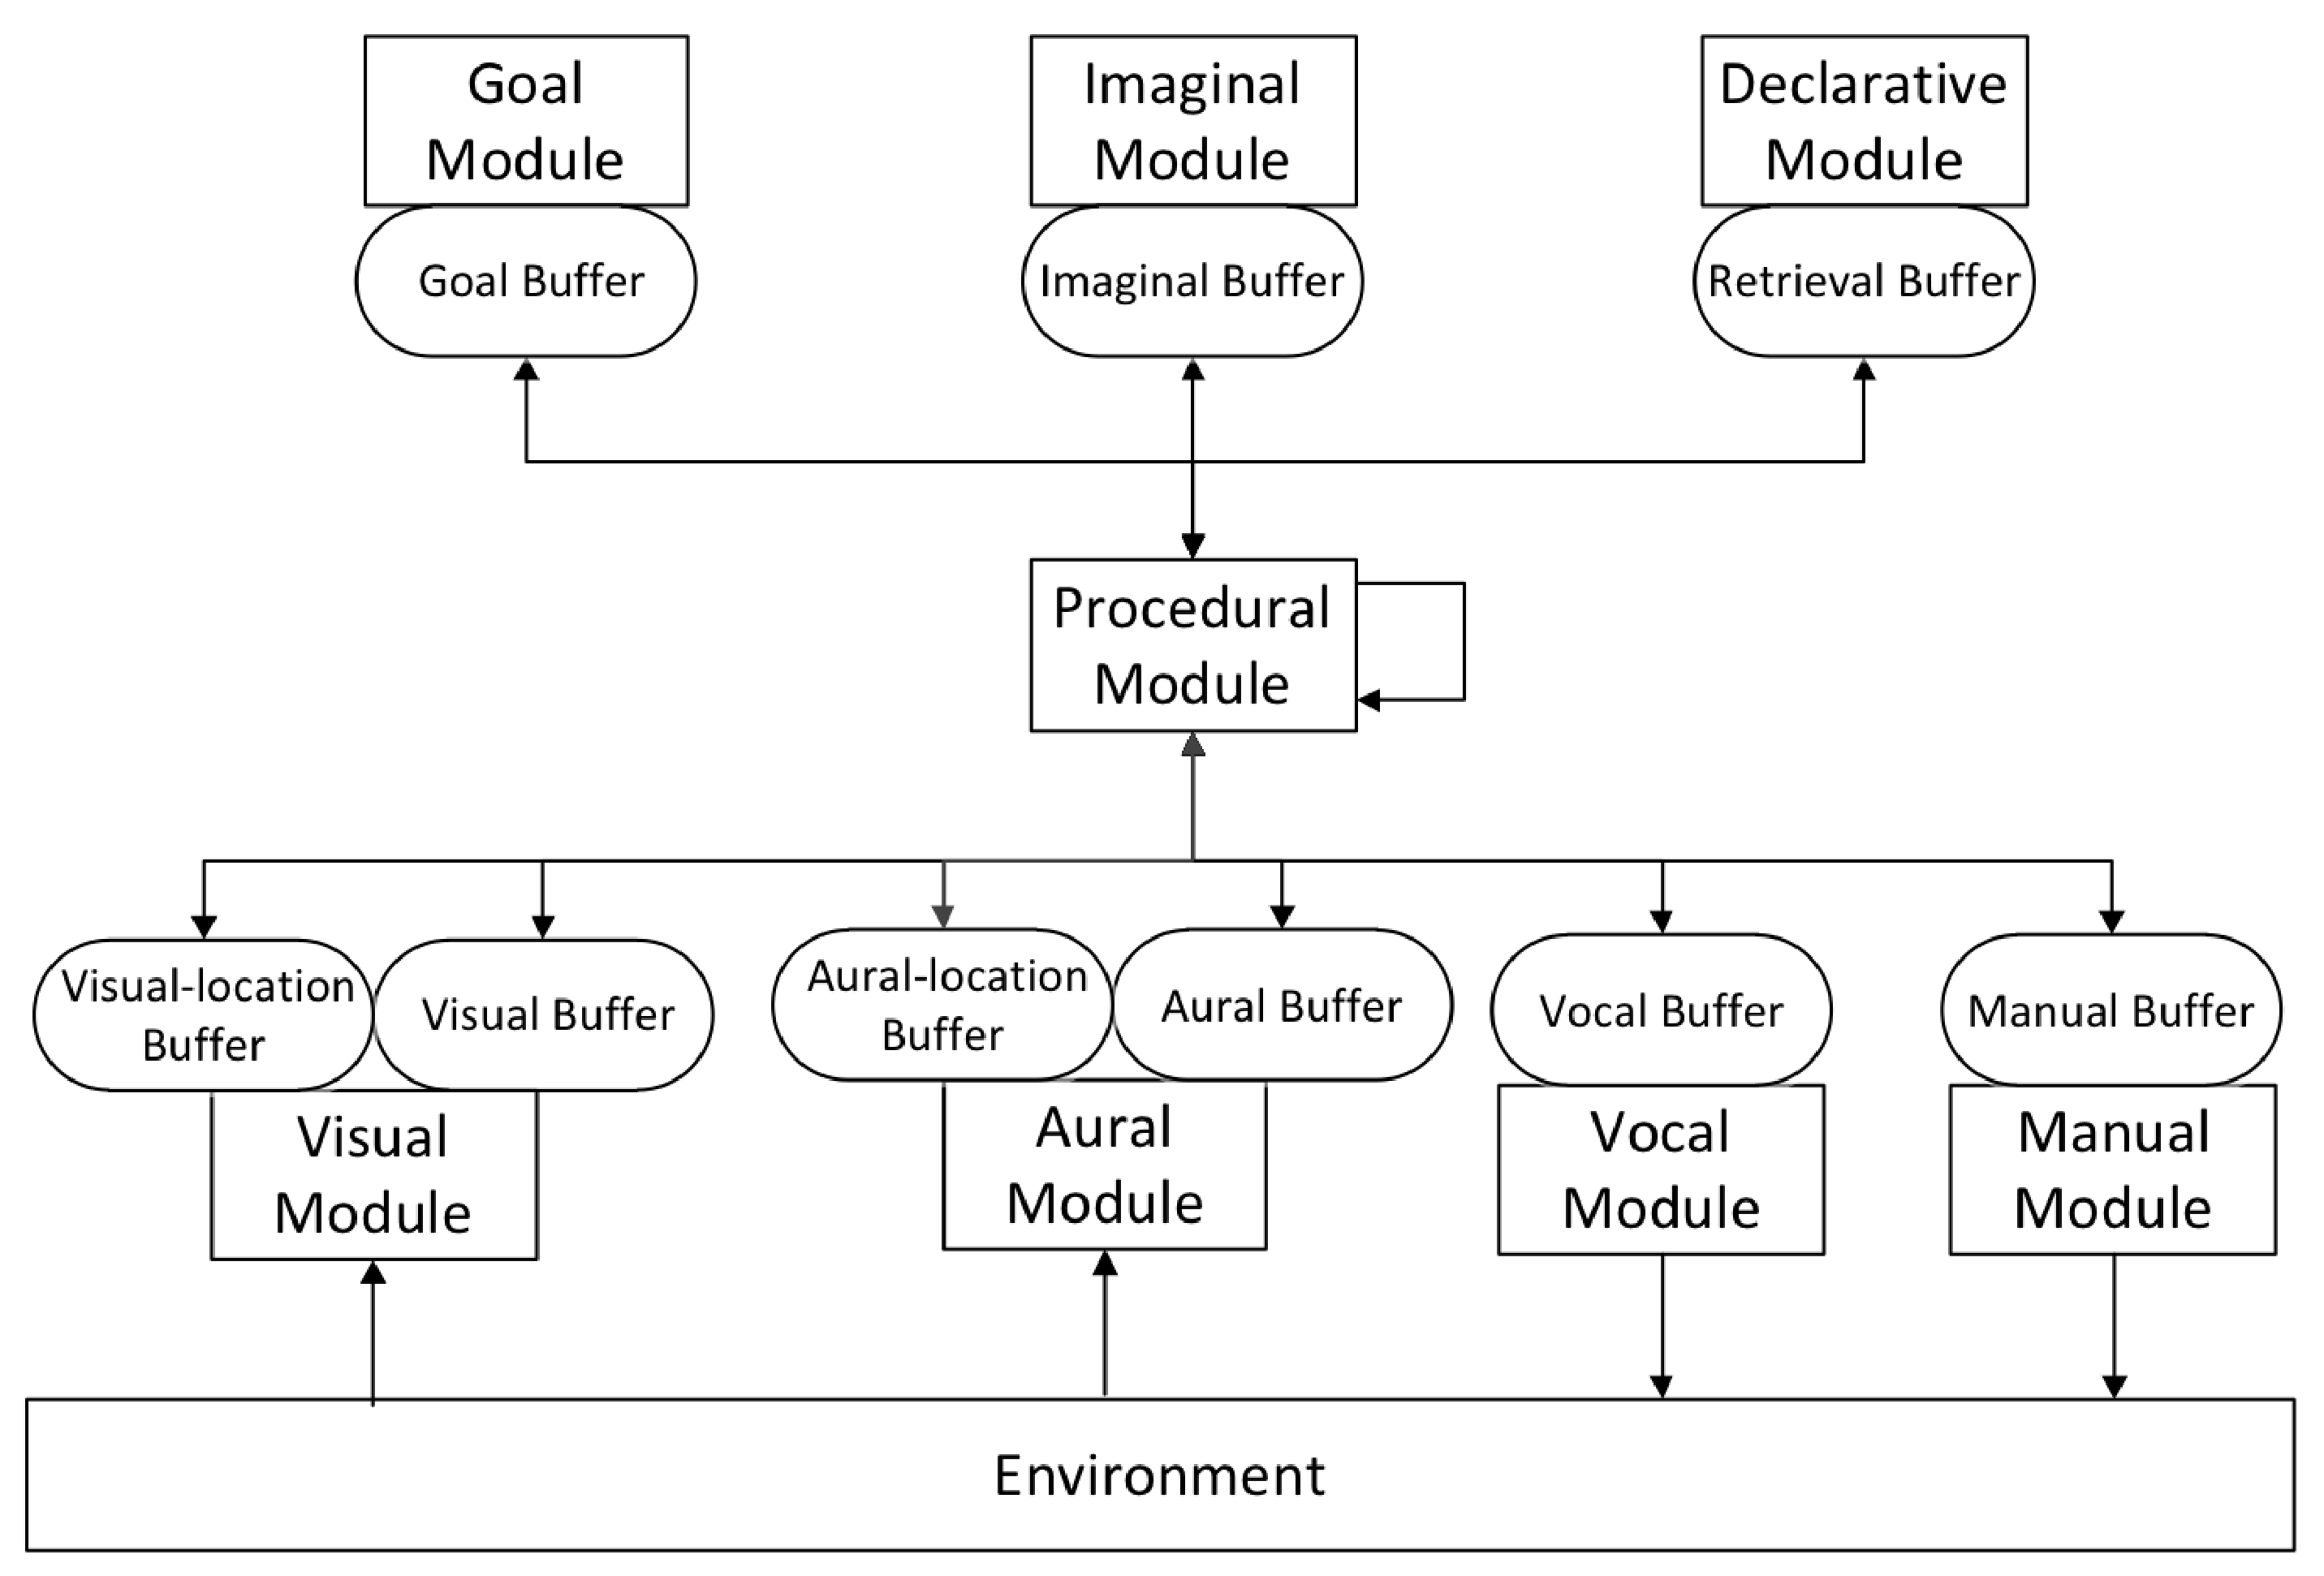
\includegraphics[scale=0.25]{images/ch_01/actr.eps}
		  \end{center} 
		  \caption{\textit{Structure of ACT-R.}}  
		  \label{fig:modulesActr}
		\end{figure}
	
	
		All the modules are independent of each other, they do not share variables or information. They can communicate with each other through \emph{buffers}, which represent the interface of a module towards the others. A module can have no buffers as well as one or more than one. The communication consists in exchanging chunks. Each module can read chunks from every buffer but it can make changes only to the chunks in its own buffers. Moreover each buffer can hold one chunk at a time. 

		Although modules usually work in a parallel way, their interactions can be only serial.
		There are two reasons for this limitation: the first one is that the structure of the buffers can hold only one chunk at a time and the second one is that only one production can be fired at a time~\cite{actr6refman}.
	
	\subsection{ACT-R Models}\label{modelSect}
	ACT-R is able to perform several task-independent reasoning. 
	To adapt these reasoning to a single task it is necessary an additional layer called \emph{model}.

	Each model contains the specific modelers' assumptions about the task within ACT-R view of cognition. That knowledge is expressed through productions that, when the model is running, interact with the modules, querying them and reading their buffers. 
	
	Running a model produces a series of atomic cognitive operations which step-by-step leads to the solution of the task. Each operation is associated with quantitative and qualitative measures like the correctness of the goal and the time necessary to complete the operation.
	This fact gives the model the possibility to predict the sequence of cognitive actions produced by human beings when they try to solve the same task.
	Comparisons with human performances can be useful to evaluate the quality of the models~\cite{Sears2012}.

	ACT-R is written in Lisp and provides its own lisp-like language for the modelers to write the models.



		

	%TODO allungare (di parecchio)	questa parte
  %% OPENCV
  \section{OpenCV}
	\mbox{OpenCV}, an abbreviation that stands for \emph{Open Source Computer Vision}, is a computer vision library that was originally developed by Intel and, later on, by Willow Garage.
	It is a cross-platform library and can run under Linux, Windows and Mac OS X. 
	It is released under a BSD license, thus it is free and open source. 
	In the beginning it was developed in C and C++ and afterwards it was expanded by the addition of interfaces for other languages as, for example, Java, Python, Ruby and Matlab. 

	\mbox{OpenCV} is designed for computational efficiency and with a strong focus on real-time applications. On Intel architectures there is the possibility to further optimize the library thanks to Intel's \emph{IPP} library. IPP library, that stands for \emph{Integrated Performance Primitives}, contains a series of low-level optimized routines in many different algorithmic areas. If this library is installed, \mbox{OpenCV} uses it automatically at runtime.

	\mbox{OpenCV} offers a simple to use infrastructure that helps programmers create quite complicated vision applications in an acceptable time. The version 2.4 has more than 2500 algorithms that cover many areas of vision. The library has been used in many applications as, for example, mine inspection and robotics. 
	It also contains \emph{MLL}, a full and general purpose \emph{Machine Learning Library}, which provides functions for pattern recognition and clustering~\cite{bradski2008learning,OpenCV:MainWebPage}. 

	The following sections contain an introduction to computer vision, a brief history of OpenCV library, a description of its main features and an overview of its architecture. 
	%The aim of this work is not to list and describe all the algorithms and techniques implemented in the computer vision library. 
	For more information about computer vision see texts by Trucco~\cite{trucco1998introductory} for a simple introduction, Forsyth~\cite{forsyth2011computer} as a comprehensive reference, and Hartley~\cite{hartley2003multiple} and Faugeras~\cite{faugeras1993three} for how 3D vision really works.

	
	\subsection{Introduction to Computer Vision}
	Computer vision is the transformation of image or video data into a new representation. Such representation can be either another image, for example a gray-scale version of the original one, or even a decision based on the information extracted from the input data. 
	Often computer vision algorithms use contextual information in order to simplify the problem.

	People not expert in computer vision may mislead the complexity of its tasks. Often, in fact, even a very simple operation for the human brain, like recognizing an animal in a picture, represents a very complex task for a machine. 
	Human visual system is very complex. It divides the visual signals into many channels, each of which brings a different kind of information to the brain. The brain uses an attention system which identifies important parts of the image and focuses on them, excluding the analysis of the remaining parts. Moreover, further information coming from all the other senses and the experience acquired during the whole life of the person completes the analysis of the image, in a way still not completely understood. All these factors create the visual perception of human beings.

	In a machine vision system, instead, when the computer receives an image or a video from a camera, it receives simply a grid of numbers. In most of cases, there are no mechanisms for pattern recognition, automatic control of aperture and focus of the camera nor cross-associations with other senses or experience.  
	Figure \ref{fig:imgMatrix} explains this concept. The machine does not recognize automatically the side mirror of the car, it sees just a grid of numbers. A goal of computer vision is to turn the grid that describes this particular object into the object itself. 
	
	
	\begin{figure}[h]
	  \begin{center} 
	    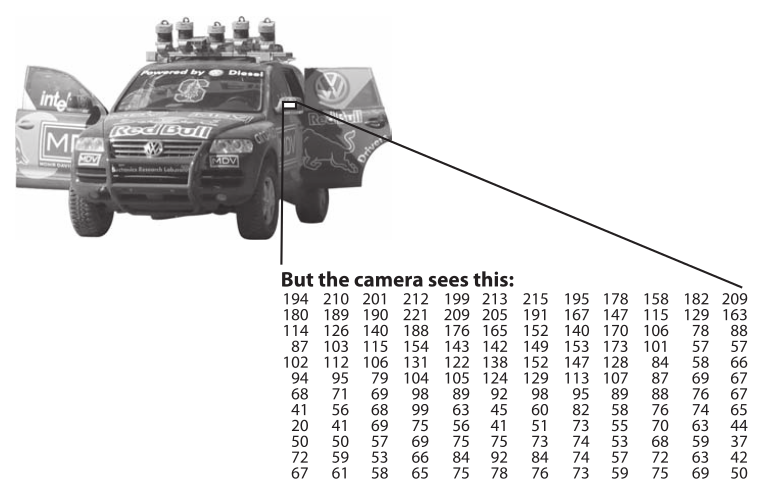
\includegraphics[scale=0.6]{images/ch_01/img_matrix.png}
	  \end{center} 
	  \caption{\textit{Representation of an image in a computer vision system.}}  
	  \label{fig:imgMatrix}
	\end{figure}

	Figure \ref{fig:2d3d} shows another aspect that makes computer vision tasks so difficult to solve. An image is a 2D description of a 3D world. The problem in the way it is posed is impossible to solve. There are infinite possible ways to reconstruct a 3D world from a 2D image. As shown in the picture, the solution changes with the point of view of the camera. This is formally an ill-posed problem.

	\begin{figure}[h]
	  \begin{center} 
	    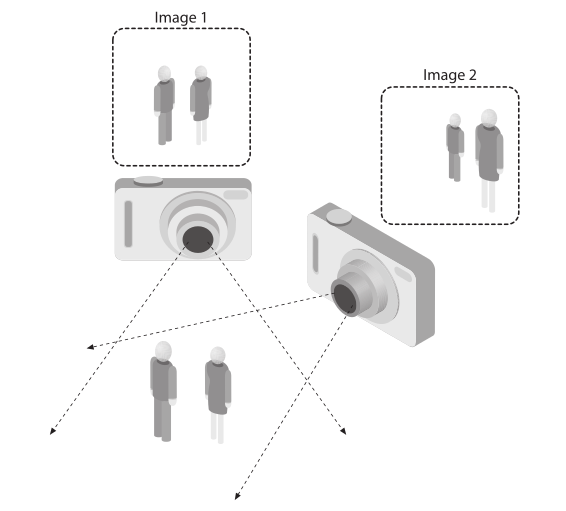
\includegraphics[scale=0.6]{images/ch_01/2d_3d.png}
	  \end{center} 
	  \caption{\textit{How the 2d representation changes with the viewpoint}}  
	  \label{fig:2d3d}
	\end{figure}

	Moreover, generally speaking, data is affected by noise. The word noise comprehends all the possible variations in the world, like weather, lightning, reflections and movements, and all the imperfections affecting the input mechanisms, like errors of the lens or of the sensors. 
	
	Some causes of noise are easy to remove. The errors caused by the lens, for example, can be mathematically described by polynomial functions, thus it is quite simple to correct them. 
	The environment variations, instead, are not well known a priori, hence are more difficult to delete. Typically, this category of noise is dealt with statistical methods, that generally do not remove it completely but attenuate it. Say, for example, to have many different pictures of the same visual scene, every one taken in different conditions of weather, lightning, reflections and so on. In this case the noise is considered, statistically speaking, a white noise. A statistical approach suggests to make the average of all the pictures. In this way, the features of the image remain, while the noise is reduced by the average operation.
	
	A common way to simplify the problem of computer vision is to add contextual knowledge to the solution. 
	Consider the example of a mobile robot which has to find and pick up staplers in a building. The robot can use the fact that the staplers are always on desks. This fact gives the robot an implicit information about the size and the position of the object, that brings it to exclude false "recognitions". Moreover, if all the desks have rectangular shapes, are made of wood and have the same color, the computer vision system can use this additional information to exclude other false staplers, increasing the accuracy of the research. As general rule: \emph{"the more constrained a computer vision context is, the more we can rely on those constraints to simplify the problem and the more reliable our final solution will be"}~\cite[5]{bradski2008learning}. Of course, in this way, the solution is not general purpose any more.
	
	Machine learning techniques allow to extract variables that model contextual information from a limited number of training cases and using them to solve other instances of the modeled problem. 
	Differently from the previous example, such variables are not set a priori by the modeler but are learnt from a series of trials. For this reason they can be hidden parameters or may even not represent physical quantities and remain mathematical variables~\cite{bradski2008learning}.

	\subsection{OpenCV History}
	The \mbox{OpenCV} Project starts in 1999 as an Intel Research initiative aimed to improve CPU intensive applications as a part of projects including real-time ray tracing, which in computer graphics is a particular technique for generating images, and 3D display walls. The early goals of the project are: developing optimized code for basic vision infrastructure, spreading this infrastructure to developers and making it portable and available for free, using a license that allows the developers to create both commercial and free applications.

	The first alpha version is released to the public in 2000, followed by five beta versions between 2001 and 2005, which lead to version 1.0 in 2006. In 2008, the technology incubator Willow Garage begins supporting the project and, in the same year, version 1.1  is released.

	In October 2009, \mbox{OpenCV} 2.0 is released. It includes many improvements, such as a better C++ interface, more programming patterns, new functions and an optimization for multi-core architectures. According to the current \mbox{OpenCV} release plan, a new version of the library is delivered on a six-months basis~\cite{OpenCV:ChangeLogs}.



	\subsection{Main Features}
	\mbox{OpenCV} offers a wide range of possibilities. First of all, it provides an easy way to manage image and video data types. It also offers functions to load, copy, edit, convert and store images and a basic graphical user interface that allows the developers to handle keyboard and mouse and display images and videos. The library permits to manipulate images even with matrix and vector algebra routines. It supports the most common dynamic data structures and offers many different basic image processing functions: filtering, edge and corner detection, color conversion, sampling and interpolation, morphological operations, histograms and image pyramids. Beyond this, it integrates many functions for structural analysis of the image, camera calibration, motion analysis, object recognition and machine learning~\cite{Agam2006}.

	%\todo{espandere (dopo aver scritto la parte di architettura)}
	
	\subsection{Architecture}
	Since version 2.2, the \mbox{OpenCV} library is divided into several modules, built in library files. Each module serves a specific purpose and includes functions in order to accomplish it. 
\begin{comment}	
The modules are:
	\begin{itemize}
	    		\item the \emph{core module}, that contains the core functionalities of the library, i.e. the basic data structures and functions used by all the other modules. The functions 
			\item ;
			\item ;
			\item .
	\end{itemize}
\end{comment}

	The \emph{core module} contains the core functionalities of the library, i.e. the basic data structures, both in C and \mbox{C++} languages, and a variety of functions used by all the other modules. Such functions have many purposes: operating on arrays and matrices, drawing shapes on the images, storing and restoring library data structures and primitive data types in \mbox{XML} and \mbox{YAML} formats and other.
	
	The \emph{imgproc module} contains the main image processing functions. Processing an image means \emph{"using higher-level operators that are defined on image structures in order to accomplish tasks whose meaning is naturally defined in the context of graphical, visual images"}~\cite[128]{bradski2008learning}.
	Such functions are, for example, operations to perform various linear or non-linear filtering on 2D images, geometrical transformations of 2D images (resize, affine and perspective warping, generic table-based remapping), color space conversions, histogram analysis, feature detection and object detection.
	
	The \emph{highgui module} allows the library to interact with the operating system, the file system and hardware such as cameras. Its interface permits to open windows, display images, read and write graphics-related files, both images and video, and handle simple mouse, pointer, and keyboard events. It also allows to add simple user interface elements to the displayed windows.   

	The \emph{features2d module} allows to use different algorithms to implement the \emph{interest points processing}. This technique relies on the idea that instead of analyzing the complete image it is better to work on a limited number of particular pixels. Such points must be distinguishable features in all the images in which they must be detected. 
	To do this, the module offers functions for feature detection, feature description and descriptor matching.

	The \emph{calib3d module} focuses on camera calibration and stereo vision. Camera calibration permits to modify images and videos by correcting the errors derived by the use of lenses. Stereo vision allows to have benefits from all the advantages given by using two equal cameras instead of one, like for example measuring distances with high precision.

	The \emph{video module} implements some techniques for video processing, in particular \emph{motion estimation}, \emph{feature tracking}, and \emph{foreground extraction} algorithms. Motion estimation techniques define motion vectors that describe the transformation from consequent frames. Feature tracking algorithms improve motion estimation by working only with some features instead of sets of pixels. Foreground extraction algorithms try to recognize foreground objects of interest comparing an observed image with an estimate of the same image as if it contained no objects of interest. 

	 The \emph{objdetect module} allows the detection of particular categories of objects such as faces or cars. To do so, it uses functions for training the software in recognizing a particular class of objects and verifying if an input image contains such kind of object once the learning is terminated. 

	\mbox{OpenCV} also includes other utility modules: the \emph{ml module} contains machine learning functions, the \emph{flann module} computational geometry algorithms, the \emph{contrib module} some contributed code, the \emph{legacy module} some obsolete code and the \emph{gpu module} support for gpu acceleration ~\cite{laganiere2011opencv,OpenCVDoc,bradski2008learning}.



	\newpage
	\chapter{Objective}\label{chObjective}
	In the first section the chapter introduces the purposes of the working team and motivates the choices of the objectives of the software. Then, in the second one, it presents the goals of the software and, in the third, the requirements.
 
\begin{comment}
The objective of the work is composed by the goals the software have to reach and the definition of the requirements for achieving them. These two aspects are described in the following sections.
\end{comment}

	\section{The Context}
	The work presented in the following chapters is a subset of the work of a research group, which aims to provide \mbox{ACT-R} of a visual system which is as similar as possible to the human one. 
	As this objective is very broad, this work focuses only on a particular subset of tasks.

	%As this goal is very ambitious and the author of this document has been introduced in a team with specific sub-goals only for a limited amount of time, he focused on particular tasks. Such tasks are described in the next sections.

	%The final purpose of this work is to provide \mbox{ACT-R} of a complete visual system, which is as similar as possible to the human one. 
	%This fact represents a huge challenge for the research world. 
	To reach such goal, the researchers continuously monitor the progresses in the computer vision research field in order to find useful innovative techniques to combine with consolidated solutions. 
	Such search, anyway, it is not easy. In fact, although computer vision studies are very active and find every year new algorithms able to solve different problems, often such algorithms introduce contextual information that makes them tasks specific: they are suitable to solve only the specific tasks for which they are designed. 
	For this reason, it is very difficult to find a general purpose solution which is able to make machine vision system behave like the human one.


%	Like most of research works, this project requires an unknown time to produce final and acceptable results.
	Like most of research works, this project has to deal with a certain degree of uncertainty that makes difficult to set any time constraints.
	The author of this work, however, has been inserted for a limited time interval in a team composed by three people, whose aim is to implement particular solutions in order to solve specific tasks. 
	For this reason the following parts of this document describe only the features developed during this amount of time by the author, explaining them in the context of the objectives of the team. 
	
		\subsection{The Goal of the Team}\label{goalTeam}
		The goal of the team is to create a general purpose software, which receives as input a video stream or an image and performs an object recognition process.
		\mbox{ACT-R} uses the information obtained by this tool to orientate inside a building.
% by distinguishing different categories of rooms thanks to the objects they contain.
		In particular, the software analyzes a video looking for objects and transmits all the recognized items to a model developed in \mbox{ACT-R}. The model has to distinguish different categories of rooms basing on the information about the objects they contain.

		As a starting point for such software, the team has to implement a tool for recognizing geometrical shapes in the input images. Such software has to accomplish two goals: the first one is to extract a subset of all the features in the image, in order to simplify the object recognition process; the second one is to make easier the definition of models for the modelers. This tool, which represents the main topic of this work, is described better in the next sections. 
%\end{comment}
		

%\todo{sistemare}
\begin{comment}
		The goal of the team is to create a general purpose software, which receives as input a video stream and performs an object recognition process. 
		\mbox{ACT-R} uses the information obtained by this tool in combination with its intelligence to orientate a robot inside a building and drive it through the structure. The robot has a camera mounted on it that transmits the video stream to the object recognition tool. This instrument analyzes the video looking for objects and transmits all the recognized ones to the artificial intelligent framework, that takes all the decisions necessary to drive the robot. 
	
		As a starting point for such software, the team has to implement a tool for recognizing geometrical shapes in the input images. Such software has to accomplish two goals: the first one is to extract a subset of all the features in the image, in order to simplify the object recognition process; the second one is to make easier the definition of models for the modelers. This tool, which represents the main topic of this work, is described better in the next sections. 
\end{comment}

	\section{The Goals of the Software}\label{TeamGoal}
	The software to be designed and developed is a visual module for the cognitive architecture ACT-R, whose aim is to improve ACT-R visual perception in order to make it more similar to the human one. 
	
	In order to develop a model in ACT-R, the modelers need a series of parameters on which basing their assumptions about the model itself and its performances.
	The collection of such data is accomplished thanks to experiments in which human beings take part. 
	For every experiment a specific program is created in order to measure some variables as, for example, the time needed to complete a task and the accuracy of the result.
	The parameters obtained by these experiments are then used as a reference for the development of ACT-R model.

\begin{comment}
After a model is developed in ACT-R, it needs to be validated . Model validations usu-
ally are realized with experiments in which human beings take part. For every experiment
a specific program is created in order to measure some variables as, for example, the time
needed to complete a task and the accuracy of the result. The parameters obtained by
the model are then comparemd with the ones obtained in these experiments.
\end{comment}


 
	Image~\ref{fig:RushHourHuman} shows a test case of an experiment in which the goal is to solve some levels of the game \emph{Rush Hour}. As shown, the grid contains some colored rectangles, each of which represents a car. The player must free the red one making it go out of the grid through the exit on the right. The cars can be moved only in the horizontal and vertical directions, according to their orientation. %The goal of the game is to free the red car. 
	The lower the number of moves, the better is such solution.

	\begin{figure}[!h]
	  \begin{center} 
	    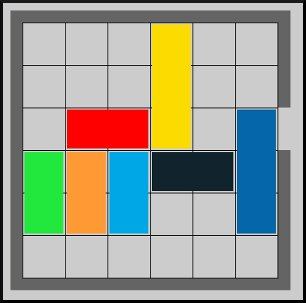
\includegraphics[scale=0.6]{images/ch_03/originale.jpg}	
	  \end{center} 
	  \caption{\textit{Example of level of Rush Hour game}}
	  \label{fig:RushHourHuman}	
  	\end{figure}
	
	In order to conduct an experiment, the modelers prepare a set of instances of the problem and every person who is going to participate to the experiment has to face a fixed number of them.
	For each instance, the ad-hoc program shows the image with the initial configuration (figure \ref{fig:RushHourHuman}) and the person has to give the solution of the game by clicking on the rectangles in the order he thinks to be correct. As the program never updates the image, the player has to imagine the solution. The software manages to interpret the direction of the shift by analyzing the movement of the eye, thanks to a module of \emph{eye tracking}. Moreover, it records the movements of the mouse, the clicks of the mouse, the time needed to give the solution and the correctness of the solution. 

	The model written in ACT-R in order to solve a particular instance of Rush Hour problem needs to receive as input the initial configuration. At the moment, such configuration is not an image, like the one shown to people during the experiment; rather it is a list of objects written in the language of the model.
	A desirable improvement of the model should be introducing an object recognition algorithm able to detect the rectangles in the image and generate the correspondent object list in ACT-R language. 
	This approach would make ACT-R visual system more similar to humans'. Moreover, it would make more scalable the process of creating instances for the experiments. 


\begin{comment}
	The models written in ACT-R that need to process images, like the one used to solve the rush hour game, at the moment skip the image processing step and start directly from a list of objects which is written directly in the input of the model. ACT-R can not accomplish this task because its visual module does not provide functions for the image processing.
	This fact represents a big limitation for the architecture and leads to a significant gap between the human cognitive system and the framework one. In addition, writing the objects in a model leads to other problems as, for example, the loss of time to write the object for every single test, the consequent delay of the work and the non-scalability of this approach.
\end{comment}
	
	%The goal of the developed software is to reduce the gap between the human and ACT-R visual systems, being a starting point for a complete and general purpose tool for the cognitive architecture to recognize objects. 
	The purposes described above represent the goals of the tool.
	To achieve them, the software analyzes the image created for the user, processes it extracting the features needed by \mbox{ACT-R} and stores the information in dedicated data structures. Then, when \mbox{ACT-R} requests them, it communicates all the stored data to the cognitive architecture using a format compatible with \mbox{ACT-R} model. 
	

\begin{comment}
	The goals of the software  are to simplify the psychologists work of defining new test cases for experiments in ACT-R and to recognize objects during the navigation of robots.

	At the moment, a psychologist, in order to insert a new test in ACT-R, has to create two interfaces, one for the user and one for ACT-R.
	The interface for the user is generally an image and can be created with any graphical editor. 
	The interface for ACT-R, instead, is much more complicated and requires the creator of the experiment to write each shape directly on the visual buffer. \todo{check correctness of this} \todo{check if the visual buffer has been introduced}
	
	The following picture shows an example of the two images used in the test.
	The one on the left is the image shown to the user while the image on the right represents the ACT-R one. 
		
	\begin{figure}[h]
	  \begin{center} 
	    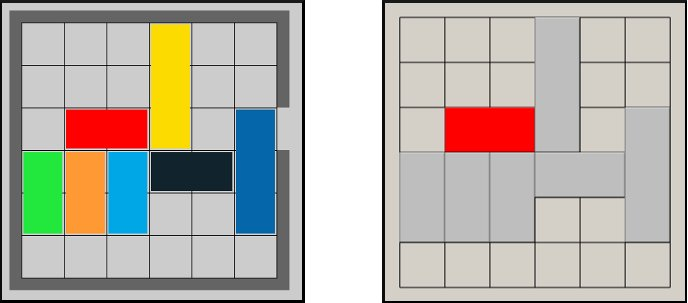
\includegraphics[scale=0.6]{images/ch_03/original_and_visicon.jpg}
	  \end{center} 
	  \caption{\textit{The two versions of the image: on the left the image for the use, on the right the image shown in ACT-R}}  
	  \label{fig:OriginalAndVisiconImages}
  	\end{figure}

	

	So, to create a test, the psychologist has to create the same image in two different formats.
	This double work causes a loss of time for the psychologist. Moreover, writing by hand all the shapes on ACT-R visual buffer is a low-level activity and can lead to stress and consequently to errors.


	The purpose of the software is to avoid to the psychologists the activity of writing on ACT-R visual buffer. To achieve this, the software analyzes the image created for the user, processes it extracting the features needed by ACT-R and communicates them to the artificial intelligence framework, which designs them automatically on its visual buffer. 
	This relieves the creators of the test of the double task described above leading to a better working experience, a less stressed work and a lower probability of errors.
	

	\todo{will i put this? or will i put it in the future developments? at the beginning it was a requirement. Will i say that the object recognition part is not developed yet?}
\end{comment}


	\section{Requirements}
	The requirements are grouped in the following sections according to the functional/non-functional classification. 
	%The simple shapes recognized are circles, triangles, squares, rectangles and ellipses.
	%Another important feature that must be introduced is the recognition of the text

		\subsection{Functional Requirements}
		The objective of the work is to design and implement a standalone software module which receives as input an image and is able to analyze it and extract some features of it.

		The input image is a color image which contains simple shapes. The shapes must not be overlapping and must have the same color hue.

		The software must recognize simple shapes, in particular:
		\begin{itemize}
	    		\item triangles;
			\item rectangles;
			\item quadrilaterals;
			\item circles.
		\end{itemize}

		For each shape, it must calculate:
		\begin{itemize}
		    	\item area;
		    	\item perimeter;
			\item dimensions;
			\item rotation;
			\item a rectangular bounding box;
			\item center;
		\end{itemize}

		Moreover, the software has to:
		\begin{itemize}
			\item recognize the color of a single pixel;
			\item recognize the color of a shape;
		    	\item calculate distances between objects;			
			\item make dimensional comparisons between objects;
			\item calculate the relative position of one object in respect with another one.
		\end{itemize}

\begin{comment}
		The shapes to be recognized are circles, triangles, rectangles and squares. 
		The color of the object is calculated averaging all the pixels of the object.
		The rotation is defined as the angle between the less sloped segment of the boundary of the object and the horizontal direction, calculated in the counterclockwise order.
		The bounding box is a rectangle whose coordinates are calculated getting the minimum and the maximum coordinates in the horizontal and vertical directions of the pixel of the image. 
		The center of a shape is the center of the bounding box.
		The distances between objects are calculated in two different ways. The first one is the distance between the centers of two shapes. The second one is the minimum distance calculated between each vertex of the bounding box of the first shape and all the vertexes of the bounding box of the second shape.
		The dimensional relation between two objects is made comparing their areas. 
		The relative position of two objects is found comparing the positions of the two top-left vertexes of each bounding box.
\end{comment}

		The software must be able to communicate with ACT-R. 
		In particular, ACT-R must signal to it which is the image to process and ask for the features to be extracted. The module must return all the information extracted by ACT-R.

		\subsection{Non-Functional Requirements}

			\subsubsection{Product Requirements}
			The software module must:
			\begin{itemize}
				\item be multi-purpose;
				\item be portable;
			    	\item work in background;			
				\item communicate with \mbox{ACT-R}.			
			\end{itemize}
			

				\paragraph{Multi-Purpose}

				The software should be easily adapted to work with all the experiments that will be put in place in the future. Moreover, there should be the possibility to adapt the software in order to use it as a shape recognition tool in the navigation with robots. For this topic, see~\ref{goalTeam}. 				
			
				\paragraph{Portability} 
				The software has to work on several operating systems.
			
				\paragraph{Communication with ACT-R} 			
				The software must transmit the extracted information to \mbox{ACT-R} in a standardized format.

%must try more than one solution and find the simpler way to integrate the software developed with the remaining architecture.
			
			\subsubsection{Organizational Requirements}
			\begin{itemize}
				\item The language of the implementation of the software must be C++;
				\item the computer vision library to be used must be OpenCV;
			    	\item a strict monitoring of the work is required.					
			\end{itemize}
		

\begin{comment}
		\subsection{Non-Functional Requirements}
		The non-functional requirements described in the following subsections are respectively the requirements on the product and the organizational ones.

			\subsubsection{Product Requirements}
			The software module must be multi-purpose, portable, must work in background and communicate with \mbox{ACT-R}.

			

			As portability is intended that it has to work on more operative systems.

			
	
			\subsubsection{Organizational Requirements}
			 
			
			%The adopted version control system must be Git.
			
\end{comment}


%	\section{Future Development}\label{futureDev}
\begin{comment}
		Another scope in which the software will be used is the robot navigation. 
		The shapes identified by the software will be used like a starting point for an object recognition process. 
		The information about these objects, then, will be used by ACT-R in order to take intelligent decisions during the robot navigation inside a building, without any other knowledge of the environment. 
		The object recognition module has not been developed yet nor the requirements for achieving this second goal are defined. 	

		Moreover, in order to scale with other kinds of experiments an \emph{optical character recognition} tool will be added and other simple shapes will be recognized.
\end{comment}
\begin{comment}
		The applications of such tools are various. 
	It is enough, for example, to add the robot a particular instrument for grabbing things and the necessary intelligence to \mbox{ACT-R} for managing such tool in order to make the robot bringing objects from a place and moving them to another. With the necessary intelligence, the robot could play chess, cards or other games. 
	
	

	Another scope in which the software will be used is the robot navigation. 
	The shapes identified by the software will be used like a starting point for an object recognition process. 
	The information about these objects, then, will be used by ACT-R in order to take intelligent decisions during the robot navigation inside a building, without any other knowledge of the environment. 
	The object recognition module has not been developed yet nor the requirements for achieving this second goal are defined. 	

	Moreover, in order to scale with other kinds of experiments an \emph{optical character recognition} tool will be added and other simple shapes will be recognized.
\end{comment}	



\begin{comment}
	\section{Functional Requirements}
		The objective of this work is to make easier the creation of an ACT-R test.\newline
		At the moment, a psychologist, in order to create a test, has to create two interfaces, one for the user and one for ACT-R. The user interface is quite simple, it is formed by simple shapes that can have different colours and words. The user has to read or watch the screen and then choose between a series of possibilities. In order to be analysed by ACT-R, this interface must have a corresponding one, which is simpler and contains only the most important features of the first one. This "simpler" interface is given as input to ACT-R and is written according to a fixed pattern. The figure below shows an example of the user interface of a test and of its corresponding one.\newline \newline	

			%qui metterei le due figure


		The purpose of this work is to create a module which is able to receive as input the user interface, recognize the main features in it and create the corresponding ACT-R interface, which must contain only such features. In order to do this, the software must be made by two parts. The first part will analyze the image. It will recognize and distinguish simple shapes, such as squares, rectangles, circles, stars, arrows; distinguish the colours of the objects; determine the position of each object in the image and recognize the text in the image. The second part will create the correspondent interface for ACT-R, thus... \newline \newline	 %% come deve fare a creare lquestai nterfaccia (lisp o qualcos altro)???? 
		  
		The software is going to be tested with several ACT-R test.
	
	\section{Non Functional Requirements}
\end{comment}	


	\newpage
	\chapter{Development Process}
This chapter, after having introduced the software development framework SCRUM, describes the development process adopted during the development.

	% TODO
	\section{SCRUM}
	SCRUM is a framework for the agile management of the project development. 
	As such, it does not define the technical way in which the developers must do the job but it follows the development process. 	
	The framework has many dimensions, roles, events, rules and artifacts, each of which within the framework serves a specific purpose and contributes the Scrum's success. The following sections describe one by one these components.

		\subsection{The Scrum Team}
		The \emph{Scrum Team} is composed of a \emph{Product Owner}, the \emph{Development Team}, and a \emph{Scrum Master}.
		These figures have different roles but all of them have to reach the same goal, deliver an increment part of usable product at constant time intervals (see \ref{Sprint Planning}). Scrum Teams are self-organizing and cross-functional. Self-organization gives the members the possibility to choose how best to accomplish their work, without being directed by others outside the team. Cross-functionality gives the team all the competencies needed to accomplish the work without depending on others not part of the team. The delivery of the products is iterative and incremental. This fact guarantees a constant feedback on the correctness of the job and ensures that a potentially useful version of the working product is always available.
			\subsubsection{Product Owner}
			The \emph{Product Owner} is the person who represents the stakeholders of the job. The Product Owner can represent the will of a committee but must be one person. His or her role is to define the requirements that the new versions of the product must have, give them the priorities, explain them to the team in detail and is responsible for the performance of the team. These requirements are called \emph{Backlog Items} and are included in the \emph{Product Backlog}. This document is described in more details in the \ref{Artifacts} section.

			\subsubsection{Development Team}
			The \emph{Development Team} consists of professionals who have to add the new functionalities to the product. The team are usually composed of three to nine members. One team must be self-organizing, this means that only the members can decide the step by step tasks to be accomplished in order to add the functionalities to the product. Every team is also cross-functional, i.e. is composed by people who have different skills. In this way it can be autonomous and it does not have to depend on other people outside the team to accomplish its job. More the Development Team's synergy is, more optimized its overall efficiency and effectiveness are.
 
			\subsubsection{Scrum Master}
			The \emph{Scrum Master} has the role to verify that Scrum is understood and put in place. He or she does this checking that everyone in the team follows Scrum theory, practices, and rules. 
			The Scrum Master is the enforcer of the rules and interacts with all the people inside and outside the Scrum Team in order to teach which interactions are useful and which are not.
			On one side, he helps the Product Owner finding techniques for managing the \emph{Product Backlog}, teaching him how to communicate in clear way with the Development Team and in understanding and practicing agility. On the other side, he coaches the Development Team in self-organization and cross-functionality, he protects it from unhelpful interruptions and keeps it focused on the tasks. 
			For this, often this role is referred as a servant-leader for the Scrum Team.


		\subsection{Events}
			Prefixed meetings in Scrum have the purpose to create regularity and hence to minimize the need for meetings not defined in Scrum, which can distract the members of the team from their tasks. In this events, different roles in the Scrum Team can interact with regularity, without the need for continuous interruptions. All the events are time-boxed, i.e. every event has a maximum duration. This ensures that only the appropriate amount of time is spent planning without waste of it.   
			
			\subsubsection{Sprint}
			The \emph{Sprint} is the primary unit of development in Scrum. It is a time-box with a fixed in advance duration. The duration can last from one week to one month. During this period of time the team creates finished portions of a product. 
	
			Each Sprint is preceded by a \emph{Sprint Planning Meeting}, where the Scrum Team defines the tasks for the Sprint and gives an estimation for the Sprint goal. It ends with the \emph{Sprint Review Meeting} and \emph{Sprint Retrospective Meeting}, where the Scrum Team respectively reviews the progress and analyses the mistakes in the Scrum method and proposes solution in order to avoid it in the next sprint. All these events will be described with more details in the next sections. 

			\begin{figure}[h]
			  \begin{center} 
				%TODO controllare copyright - http://commons.wikimedia.org/wiki/File:Scrum_process.svg
			    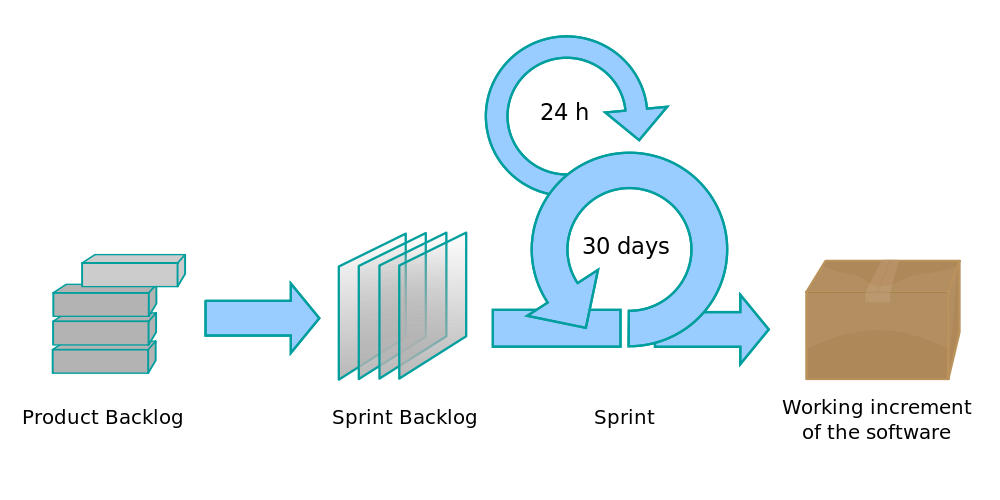
\includegraphics[scale=0.45]{images/ch_04/scrum_process.png}
			  \end{center} 
			  \caption{\textit{Overview of the Scrum Process}}  
			  \label{fig:ScrumProcess}
		  	\end{figure}


			\subsubsection{Sprint Planning Meeting}
			The \emph{Sprint Planning Meeting} is a meeting at which all the member of the Scrum Team participate. It precedes every Sprint. In this meeting the team decides which feature add to the product by the end of the Sprint.

			At first the Product Owner informs the team of the features that he wants to be completely added to the product. Every feature is an item in the \emph{product backlog}. You can find a detailed description of this artifact in the section \ref{Product Backlog}. Then, the Development Team estimates how long it takes to add every new feature to the product and, consequently, how many of them will be added by the end of the Sprint. Often this part of the meeting is signed by a clarification about the requirements between the Product Owner and the Development Team that leads to new time estimation for each goal. The goals are split into tasks, each of which takes no more than one day to be accomplished by the development team. Every task and the plan for delivery them are collected in the \emph{Sprint Backlog}. A detailed description of this document can be found in the section \ref{Sprint Backlog}.

			Every Sprint must have a \emph{Sprint Goal}. The Sprint Goal acts like a sort of motivation which reminds the Development Team during the whole sprint which is in a wider context the goal of their activities. For this the sprint goals should not be changed during the sprint.
		
			\subsubsection{Daily Scrum}
			The \emph{Daily Scrum} is a fifteen minutes event for the Development Team, that allows the team to synchronize the work and plan the next day activities. This purpose is achieved analyzing the work done in the last day and forecasting the work for the next one. 
			During the meeting, each Development Team member explains what he did since the last meeting, what he is going to do before the next meeting and the problems he has to front.
			The meeting has the purpose to evaluate the progress towards the Sprint Goal and to analyze the trend of the progress in comparison with the Sprint Backlog. 

			\subsubsection{Sprint Review}
			The \emph{Sprint Review} is a time-boxed meeting which closes every Sprint. In this meeting the increment of the work is analyzed and, if needed, the Product Backlog is updated. 
			During the meeting, the Product Owner analyzes what has been completed and what has not been completed. The Development Team describes the problem it encountered, how it solved them and shows the new functionalities added to the product. Then the whole team discusses of new opportunities and, more generally, collaborates on what to do next, updating consequently the Product Backlog.			

			\subsubsection{Sprint Retrospective}
			The \emph{Sprint Retrospective} is a time-boxed meeting which is fixed after ever Sprint Review. It is an opportunity for the Scrum Team to analyze its scrum implementation and create a plan for the improvements of the next Sprint. 
			During the meeting the focus is set on people, relationships, process and tools. The most important successes are shown and a plan for implementing potential improvements is created. 
			The purpose of this meeting is to make the implementation of the method more effective optimizing the development process and introducing techniques that make the method more productive and enjoyable. 

		
		\subsection{Artifacts}
			\subsubsection{Product Backlog}
			\subsubsection{Sprint Backlog}
			\subsubsection{Burn Down}
			
	
	
	% TODO 
	\section{The Adopted Development Process}
		%Cose che voglio dire:
		1) Processo di sviluppo incementale e iterativo
		2) No pair programmin nè test driven development  (dirlo ? )
		3) Sviluppo agile
		4) Come abbiamo usato noi SCRUM
			-) sprint: 2 settimane
			-) non c'era un committente ma c'era il project manager
			-) 1 team

\begin{comment}
	\section{SCRUM}

	\section{Working Instruments}
	In addition to ACT-R and OpenCV, many other tools have been used. Here follows a list of the most important ones.
		\begin{itemize}
		\item \textbf{Eclipse IDE for C/C++ Developers} as \textit{integrated development environment} \footnote{More informations at \url{www.eclipse.org}};
		\item \textbf{Cute} as \textit{unit testing framework} \footnote{More informations at \url{http://cute-test.com}};
		\item \textbf{Mylyn} as \textit{task and application lifecycle management} \footnote{More informations at \url{www.eclipse.org/mylyn}};
		\item \textbf{Trac} as \textit{bug tracking system} \footnote{More informations at \url{trac.edgewall.org}};
		\item \textbf{Git} as \textit{version control system} \footnote{More informations at \url{git-scm.com}}; 
		\item \textbf{Dia} and \textbf{cpp2dia} to create UML diagrams \footnote{More informations at \url{dia-installer.de} and at \url{cpp2dia.sourceforge.net}};
		\item \textbf{ZBar} to read QR codes \footnote{More informations at \url{zbar.sourceforge.net}}.
		%%It can be useful for drawing a large variety of diagrams, in particular UML diagrams, network maps and flowcharts. 
		\end{itemize}
\end{comment}

	\newpage
	\chapter{Design}
	This chapter describes the initial design of the software, that is the design thought by the team at the beginning of the development.
	For reasons of clarity, the description of the architecture follows a top-down approach and makes use of diagrams. 		The first section gives an overview of the software and the others study in deep specific aspects of it.

%	\section{How to read the chapter}
	To better explain the contents and the structure of the design, the description is supported by \mbox{UML} diagrams. The following sections describe the software at different levels of detail and the diagrams reflect this approach. In the first section, for example, they are used only to present how the classes are organized in the overall structure and for this contain only the names of the classes. Further details are added in the diagrams in the next sections, according with the top-down approach of the chapter.

\begin{comment}
	As the chosen development process is incremental and iterative as described in chapter \ref{devProcChap}, the initial design represents a reference in which are described only the well known aspects of the project. According to the agile development, the team chose to postpone the design of specific features of the software not well defined a-priori. This explains why the description does not enters into details. 
\end{comment}
	As described in chapter \ref{devProcChap}, the chosen development process is incremental and iterative.
	According to this choice, the initial design represents a reference in which are described only the well known aspects of the project. The choices regarding specific features not well defined a-priori are demanded. For this reason in this chapter the description, although it deepens specific topics, does not enter into detail. 
		
	The reader will notice that some classes that appear in the following diagrams are not described in the chapter. The reason of this is that they do not accomplish to any functions described in the requirements section of \mbox{chapter \ref{chObjective}}. Their presence makes sense in the context of the whole software, described in \ref{futureDev}. It has been decided not to remove such classes from the diagrams because they influence the project and motivate particular design and implementation choices.

\begin{comment}
The classes \emph{MarkerDetector} and \emph{QRScanner} do not accomplish to the communication with ACT-R nor the extraction of features in the way it is defined in the requirements section of chapter \ref{chObjective}. Their presence makes sense in the context of the whole software, described in \ref{futureDev}. Both of these classes work on video streams: MarkerDetector data looks for \emph{markers}, images with pre-determined patterns, and QRScanner searches for \mbox{QR} elements and tries to decode them. Both marker and \mbox{QR} elements are considered features. This fact explains the presence of these two classes in the feature extraction process. It has been decided not to remove them from the diagrams because they influence the design of the software and represent the motivations to particular design and implementation choices.
\end{comment}

\begin{comment}
	Moreover, as the software has been developed in team but this document focuses only on a subset of the whole work, some classes are shown in the diagrams but are not described. The team developed them in order to accomplish tasks fundamental in the whole context of the software but not of interest in this particular work. Such classes can not be removed from the diagrams because they influence the design.
\end{comment}

	\section{Overview of the design}
	The software is composed of four main parts, one for processing images and videos, one for containing the hierarchy of the objects recognized during such processing, one for allowing ACT-R to communicate with the software and one containing all the utility functions used by all the other parts.

	\begin{figure}[h]
	  \begin{center} 
	    \fbox{	
	       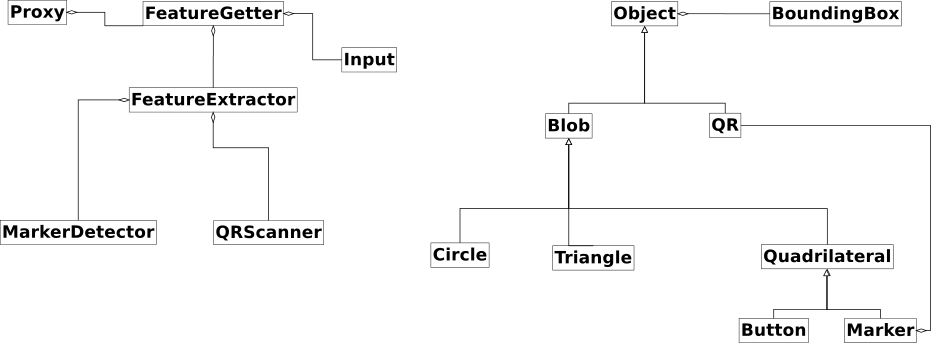
\includegraphics[scale=0.55]{images/ch_05/progettazione_overview.png}
	    }
	  \end{center} 
	  \caption{\textit{Class diagram illustrating a high level overview of the designed parts of the software}}  
	  \label{fig:swArchitecture}
 	\end{figure}		

	Image \ref{fig:swArchitecture} shows a class diagram which describes two of the parts that compose the software. 
	The part dedicated to the processing of images and video is located on the left and is composed by the classes \emph{Proxy}, \emph{FeatureGetter}, \emph{FeatureExtractor}, \emph{Input}, \emph{MarkerDetector} and \emph{QRScanner}.
	The object hierarchy, which is shown on the right, contains the classes \emph{Object}, \emph{BoundingBox}, \emph{Blob}, \emph{QR}, \emph{Circle}, \emph{Triangle}, \emph{Quadrilateral}, \emph{Button} and \emph{Marker}.

	

	The other two parts are not included in the design diagrams for different reasons. 
	According to the non-functional requirements, the team planned to try different solutions in order to implement the communication between the software and ACT-R. As different approaches can lead to different architectures, this part has not been designed a priori.
	Regarding the utility part, it depends strongly by the future design and implementations choices and is influenced by the chosen communication technique. These factor leads it to be very instable and volatile. 
	For these reasons and according to the agile development, the team decided not to spend time in planning a fixed structure for it at the beginning.

\begin{comment}
	Regarding the utility part, as it depends strongly by the implementations choices, it is very instable and volatile. Moreover, it is influenced by the chosen communication technique, which, as just described, has not been planned.
	For these reasons, according to the agile development the team decided not to spend time in planning a fixed structure for it.
\end{comment}
	
	
	\section{Feature Extraction Classes}\label{featExtraction}	
	The classes that play the role of acquiring the images and extracting features from them are \emph{Input}, \emph{FeatureGetter} and \emph{FeatureExtractor}. \emph{Proxy} has the role of intermediation between this part of the software and the one which manages the communication with \mbox{ACT-R}.

\begin{comment}
	\emph{MarkerDetector} and \emph{QRScanner} classes have been developed by the team in order to make the software locate markers and finding and decoding QR object. These tasks, although are fundamental in the whole work, are not significant in the objective of this particular work, so they are not described.
\end{comment}
	\begin{figure}[h]
	  \begin{center} 
	    \fbox{	
	       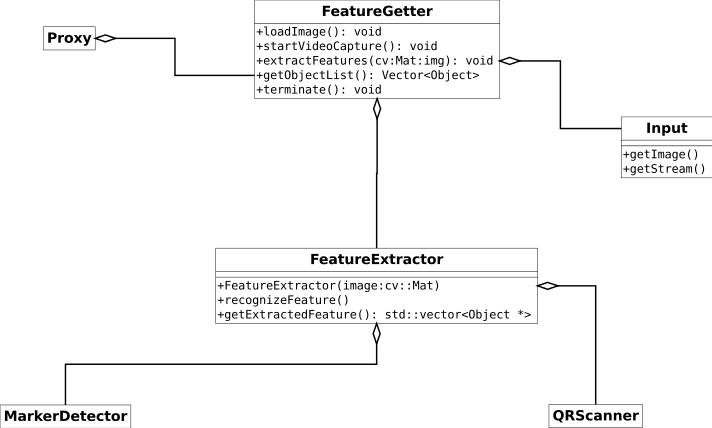
\includegraphics[scale=0.65]{images/ch_05/feature.png}
	    }
	  \end{center} 
	  \caption{\textit{Class diagram illustrating the main roles in the feature extraction process}}  
	  \label{fig:FeatureDesign}
 	\end{figure}
	
	Figure \ref{fig:FeatureDesign} contains the class diagram that designs the interface of these classes.
	\emph{FeatureExtractor} represents the core of this part. It receives in input an image and processes it in order to extract the features that contains. For each extracted feature it creates a correspondent element in the \emph{object hierarchy}. Such hierarchy is described in section \ref{classHierarchy}. Once the objects are created, the class creates a list containing all of them and delivers it to FeatureGetter. 
	FeatureExtractor is also responsible for accomplish other goals described in the requirements, like recognizing colors of pixels and objects, calculating the distances of two objects as well as the relative position of one object in respect with another one and making dimensional comparisons between two objects. These features have not been included in the initial design of the class even if it has been thought that this class would have accomplished all these tasks.

	\emph{Input} is responsible for interacting with the file system and the hardware of the computer. In particular its tasks are loading images from files, saving images to files and loading video streams from the web-cam. The acquired data are delivered to FeatureGetter. 

	\emph{FeatureGetter} represents a level of abstraction that avoids to call directly the functions of FeatureExtractor and Input, providing a simpler interface. Its functions create the Input object, receive from it the input data, delivers it to FeatureExtractor for the extraction of the features and delivers the received object list to Proxy.

	\emph{Proxy} represents a further level of abstraction between FeatureGetter and the part of the software which manages the communication with ACT-R. Most of the procedures for the communication with the artificial intelligence framework, in fact, need to use specific data types. This class has the main function to transform each object of the object list in the type necessary for the communication to ACT-R.

	For the reason explained at the beginning of the chapter, \emph{MarkerDetector} and \emph{QRScanner} are not described in this work.

\begin{comment}
	The classes \emph{MarkerDetector} and \emph{QRScanner} do not accomplish to the communication with ACT-R nor the extraction of features in the way it is defined in the requirements section of chapter \ref{chObjective}. Their presence makes sense in the context of the whole software, described in \ref{futureDev}. Both of these classes work on video streams: MarkerDetector data looks for \emph{markers}, images with pre-determined patterns, and QRScanner searches for \mbox{QR} elements and tries to decode them. Both marker and \mbox{QR} elements are considered features. This fact explains the presence of these two classes in the feature extraction process. It has been decided not to remove them from the diagrams because they influence the design of the software and represent the motivations to particular design and implementation choices.
\end{comment} 		

\begin{comment}
In this way it represents the only way in which the both It provides functions to load images, extract features from them and return a list of \emph{Object}, each of which represents one of the detected feature. 
The objects are elements of the object hierarchy, that is described in \ref{classHierarchy}. The class also allows to load a video from a webcam, extract a frame from it and apply the same algorithms to it in order to apply the feature extractions feature.
\end{comment}

	
	\section{Class Hierarchy}\label{classHierarchy}
	The class hierarchy contains all the objects that are recognized during the processing of the image. Each feature has a correspondent object that describes it. 
	
	\begin{figure}[h]
	  \begin{center} 
	    \fbox{	
	       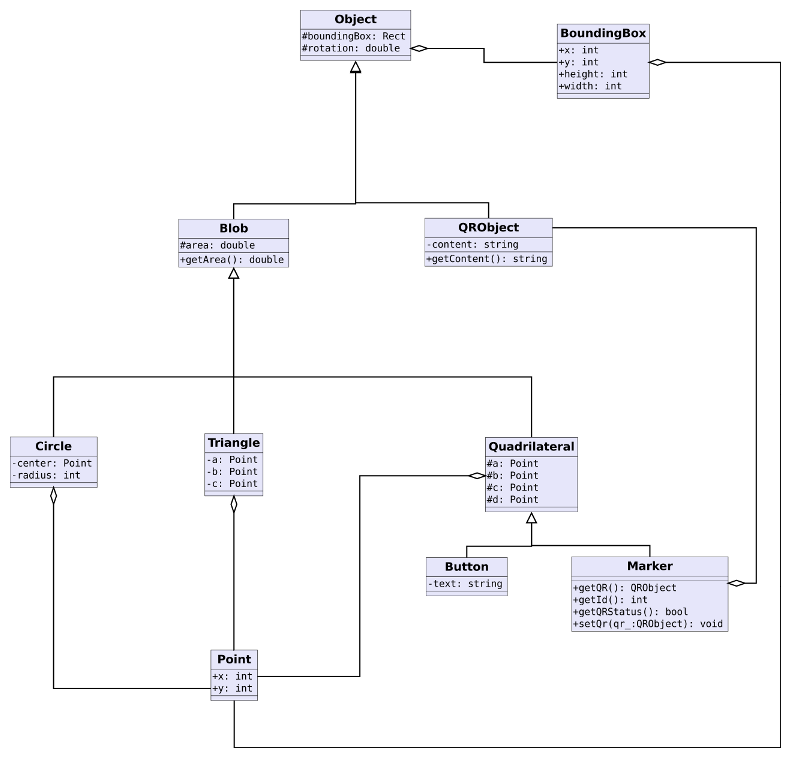
\includegraphics[scale=0.65]{images/ch_05/hierarchy.png}
	    }
	  \end{center} 
	  \caption{\textit{Class diagram illustrating the class hierarchy of the recognized objects}}  
	  \label{fig:HierarchyDesign}
 	\end{figure}

	Figure \ref{fig:HierarchyDesign} contains a class diagrams that specifies such hierarchy. 
\begin{comment}
	\emph{Object} is the superclass that represents all the possible objects recognized in an image during the feature extraction process. All the elements of this type must have a rotation value and a bounding box. The two attributes of the class \emph{rotation} and \emph{boundingBox} define such parameters. In particular, the second one has its correspondent class, called \emph{BoundingBox}. As specified in the diagram, this object can be only of rectangular shape, in fact its attributes are the coordinate of a point and horizontal and vertical dimensions.
\end{comment}
	\emph{Object} is the superclass that represents all the possible objects recognized in an image during the feature extraction process. Two attributes all the elements of this type must have are a \emph{rotation} value and a 
\emph{boundingBox}. 
	This latter parameter has a data type which is defined by the class \emph{BoundingBox}. Such element can have only rectangular shape, in fact its attributes are the coordinates of a point and horizontal and vertical dimensions.


	The type Object can be specified by two sub-types: \emph{Blob}, that represents a generic shape, and \emph{QR}, representing a \mbox{QR} element. The presence of \mbox{QR} is not important for the shape recognition task but it justifies the presence of Blob in the hierarchy. Without \mbox{QR} class, in fact, Blob could have been incorporated in Object.
	Blob is provided of the attributes \emph{area} and \emph{perimeter}, which, as suggested by the names, represent respectively the area and the perimeter of the shape.
	

	The classes \emph{Circle}, \emph{Triangle} and \emph{Quadrilateral} extend \emph{Blob}. They represent the simple shapes that can be recognized during the recognition process. Each item is defined starting by basic geometrical elements: the circle by center and radius, the triangle by three points, the quadrilateral by four points. \emph{Point} class, in particular, has been introduced in this diagram for reasons of completeness. 

	The class \emph{Button} specifies Quadrilateral by adding the attribute \emph{text}, which represents the message of such button. The fact that such class derives Quadrilateral instead of Blob reflects the requirement that the buttons can be only rectangular. 
	
	The class \emph{Marker} is not described in this document. You can find the motivation of this choice at the beginning of this chapter.


	\section{Flexibility of the design}			
	This section explains why the team designed at the beginning of the project a reference structure for the class hierarchy and the feature extraction. The two main motivations are: well defined requirements and high flexibility of such design. %The requirements are described in chapter \ref{chObjective}. Below it is discussed about such flexibility.
	
	The requirements in chapter \ref{chObjective} define precisely which are the objects, the shapes and the other features to be recognized in the images.

	The design of the class hierarchy and the feature extraction part guarantees a flexibility that allows the developers to add transparently many kind of different objects to it and introduce new features to be recognized.
	Adding further simple shapes to the hierarchy, for example, it is a task that can be accomplished easily by deriving a new type by Blob. This operation does not need to change the interface of no one of the existing classes.
	In the same way, a completely new category of object can be added simply by deriving it from Object, again without changing anything in the other classes. 
	Even the introduction of the recognition of a new feature is transparent in this architecture. It is sufficient to add a method in the FeatureExtractor class and the correspondent object, or parameter, in the hierarchy. If objects of such new kind are recognized in an image, they are added to the object list by FeatureExtractor. So nothing changes for all the other classes.

	The flexibility guaranteed by these two models allowed the developers to specify their design at the beginning of the development process.

\begin{comment} 
	
	
	\section{Communication with ACT-R}

  
  \section{The Whole Software}
  The aim of the 
  \begin{figure}[h]
	  \begin{center} 
		%TODO: aggiungere immagine	
	    %\includegraphics[scale=0.1]{images/ch_04/classDesign.jpg}
	  \end{center} 
	  \caption{\textit{Class diagram of the whole software }}  
	  \label{fig:swArchitecture}
  \end{figure}
  \todo{cambiare l immagine e aggiungere la descrizione...}.

  
  \section{The Class Hierarchy}
  \begin{figure}[h]
	  \begin{center} 
		%TODO: aggiungere immagine
	    %\includegraphics[scale=0.2]{images/ch_04/designClassObjectHierarchy.jpeg}
	  \end{center} 
	  \caption{\textit{Class hierarchy of the recognized objects}}  
	  \label{fig:callHierarchy}
  \end{figure}
   {\newpage}
   {\newpage}
   {\newpage}
   {\newpage}
  The picture above describes the hierarchy of the classes defined to contain the objects detected in the images. The \textit{Object} class represents a generic object that can be found in an image. Thus, everything which is different from the background can be seen as an instance of the \textit{Object} class. Every object must be bounded by a \textit{bounding box}. This structure is represented by the \textit{BoundingBox} class. All the bounding boxes have rectangular shape. The requirements were such that it was not necessary to define more complicate shapes \todo{migliorare questa frase, fa schifo}. The \textit{attended} attribute of the \textit{Object}  class is set to \textit{true} if the object has been already returned to ACT-R, otherwise it is set to \textit{false}. The \textit{rotation} is a value that gives the amount of the rotation in the counterclockwise directions starting from the horizontal direction \todo{controllare la correttezza}. \todo{vedere se il metodo getChunk esiste ancora}\todo{se 
non esiste eliminarlo 
dall immagine}.
  Besides the generic objects, there are two categories of object that can be found in the processed images, the \textit{QR codes} and the \textit{simples shapes}. A simple shape can be, for example, a circle, a square, a rectangle or a triangle. The QR codes is represented in the hierarchy with the \textit{QRObject} class, the generic shape with the \textit{Blob} class.
  This class has the \textit{area} parameter, which stands for the area of the object in pixel, and the  \textit{getArea} method, which returns this value. The \textit{Blob} class is realized by three classes, \textit{Circle}, \textit{Triangle} and \textit{Quadrilateral}. 
  The first one has, as parameters, the \textit{center} and the \textit{radius} of the circle itself.
  The parameters of the \textit{Triangle} and the \textit{Quadrilateral} classes are respectively three and four points, which represent the vertices of the shape. Notice that the \textit{Quadrilateral} class defines every polygon with four sides and four vertices. Thus, rectangles and squares can be instances of this class. 
  The \textit{Button} class is a realization of the \textit{Quadrilateral} class. This is because, as a requirement, buttons have always rectangular or squared shapes. The additional information they add is the \textit{text}, that is a simple message that is always present in a button. It is represented by the \textit{text} attribute. 
  The \textit{Point} class identifies a generic point in the bidimensional space. Its parameters, \textit{x} and \textit{y}, are the two coordinates in the plane.
 
  \todo{... aggiungere, correggere o finire}

  
 \end{comment} 
  
  
  

	\newpage
	\chapter{Implementation And Testing}\label{impl_test}

	\section{The architecture the software}
	As in chapter \ref{chDesign}, in this section class diagrams are used in order to clarify the description. Again, such description follows a top-down approach: section \ref{impl_arch} gives an overview of the architecture and for this reason the diagram in figure \ref{fig:implementation_names} contains only the names of the classes. The following sections study in deep specific aspects of the software and, consequently, contain more detailed diagrams.


		\subsection{Overview}\label{impl_arch}
		Figure \ref{fig:implementation_names} shows the class diagram of the whole software. 
		According to the design specifications defined in chapter \ref{chDesign}, the software is organized in four main parts, each of which has its own role.

		\begin{figure}[h]
		  \begin{center} 
		    \fbox{	
		       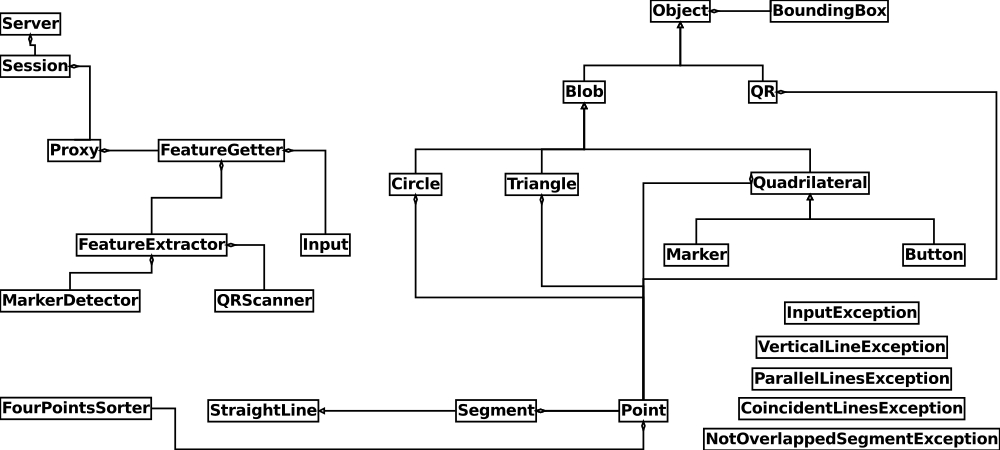
\includegraphics[width=\textwidth*\real{0.9}]{images/ch_06/implementazione_solo_nomi.jpg}
		    }
		  \end{center} 
		  \caption{\textit{Class diagram which illustrates the whole architecture of the software}}  
		  \label{fig:implementation_names}
	 	\end{figure}
 
		Classes \emph{Server} and \emph{Session} manage the communication with \mbox{ACT-R}, implemented by a client server approach.
		Classes \emph{Proxy}, \emph{FeatureGetter}, \emph{Input}, \emph{FeatureExtractor}, \emph{MarkerDetector} and \emph{QRScanner} have the role of extracting features from the input data and preparing the messages to be sent to the cognitive architecture.
		\emph{Object}, \emph{BoundingBox}, \emph{Blob}, \emph{QR}, \emph{Circle}, \emph{Triangle}, \emph{Quadrilateral}, \emph{Marker} and \emph{Button} form the object hierarchy.
		\emph{InputException}, \emph{NotOverlappedSegmentException}, \emph{ParallelLinesException}, \emph{VerticalLineException}, \emph{CoincidentLinesException}, \emph{FourPointsSorter}, \emph{StraightLine}, \emph{Segment} and \emph{Point} represent the utility classes.
	
		Comparing the classes shown in figure \ref{fig:implementation_names} with the design choices defined in chapter \ref{chDesign}, the reader can notice two facts: both the feature extractor and the class hierarchy parts strictly adhere to the project and, accordingly to the design choices, the classes containing the utility functions and the features for the communication with \mbox{ACT-R} have been properly developed.
		%The following sections presents the implementation of the whole classes, focusing mainly on these two latter parts of the software. 

	
		\subsection{Communication with ACT-R}
		\mbox{ACT-R} and the developed module use a \emph{client-server} communication mechanism based on \mbox{TCP} in order to exchange information between each other. 		

		The client-server approach has been chosen because it is standardized and supported by \mbox{Lisp} interpreters that run \mbox{ACT-R}. 
		Moreover the possibility of using shared resources and the transparency offered by the mechanism ensure very high flexibility and scalability.
		TCP has been preferred to \mbox{UDP} mainly because of the reliability guaranteed. Secondly, the communication to be implemented is bi-directional and the small quantity of data exchanged in the communication make it more suitable for the purpose.

		When an ACT-R model is run in a LISP interpreter, a second process is also launched. 

In this process all the computation related to the video and image processing is performed. When ACT-R needs to acquire information from the real world, it asks the required data. The LISP interpreter needs to communicate with the second process. The interpreter initiates a connection with the server, acting as client. Since the process of the server is running, a connection is established and the exchange of data can begin. At this stage the interpreter can encode and send a request, which will be delivered to the other process. Then the server receives the request, decodes it and requests an extraction of features.
		When the server receives a request, a feature extraction procedure starts. The position of the markers, if any, is retrieved and a video frame is analysed in order to get further informations, when needed. The exchange of information between client and server is done in a synchronous way, this means that the LISP interpreter will wait until a response is received.
		After that the response will be translated in chunks and delivered to ACT-R. After that the model will be able to continue its cognitive reasoning. All the information sent by the two parties is encoded in JSON. In the next paragraph will be described more in detail how the data are encoded.



		The part responsible for the communication with the cognitive architecture is composed by the classes \emph{Server} and \emph{Session}. 

		\begin{figure}[h]
		  \begin{center} 
		    \fbox{	
		       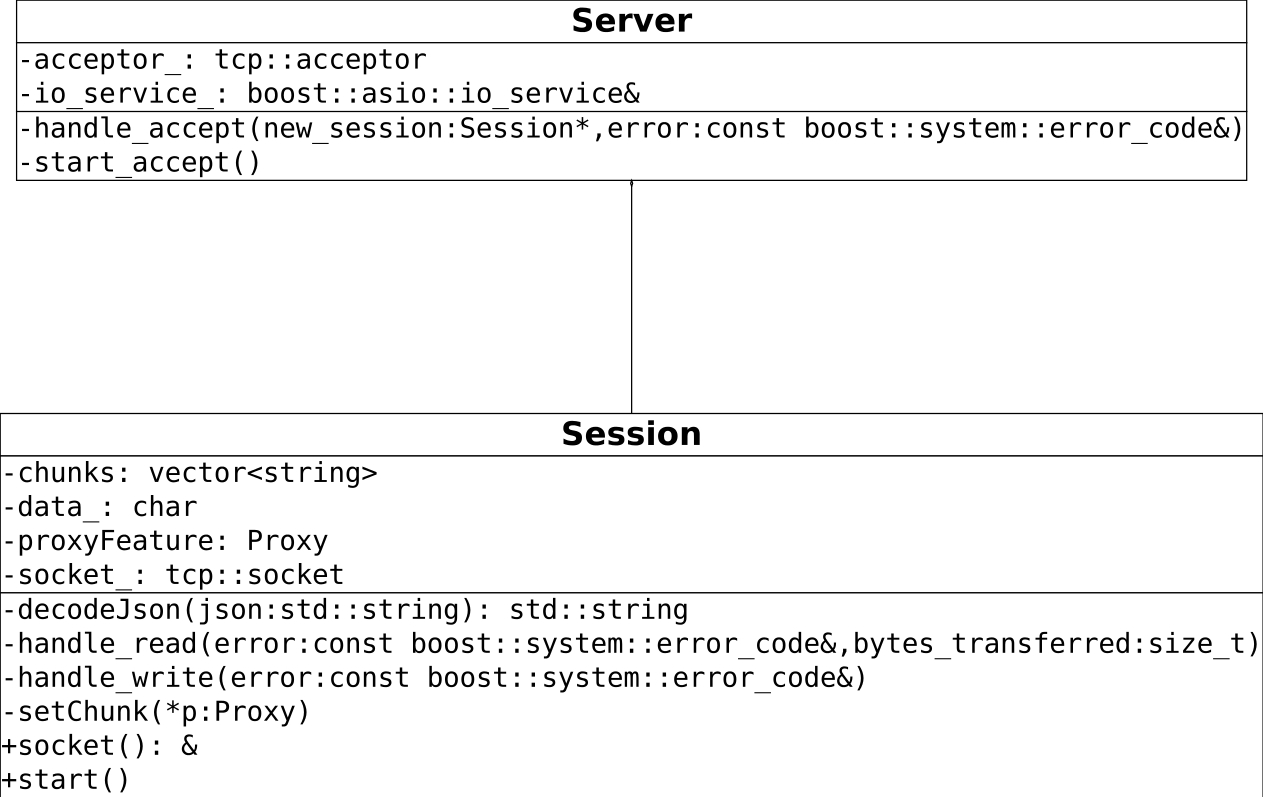
\includegraphics[width=\textwidth*\real{0.9}]{images/ch_06/communication.jpg}
		    }
		  \end{center} 
		  \caption{\textit{Class diagram describing the implementation part of the software dedicated to communication}}  
		  \label{fig:impl_feat_extraction}
	 	\end{figure}	


\newpage
		\subsection{Feature Extraction}
		Image \ref{fig:impl_feat_extraction} shows a class diagram of the implementation of the feature extractor part of the software. 
		Analyzing it, the reader can notice that the implementation adheres very good to the design specifications, described at page \pageref{featExtraction}. 
		The classes, in fact, are the same but with more attributes and methods. 
		Such additions have been introduced at development time, as the requirements became clearer.
		Notice that some methods, like for example \emph{setCroppedImage} in FeatureExtractor class, are used to obtain goals different from the one described in this work, but make sense in the general context of the team work. This topic is better explained in the introductory part of chapter \ref{chDesign}. 

		\begin{figure}[h]
		  \begin{center} 
		    \fbox{	
		       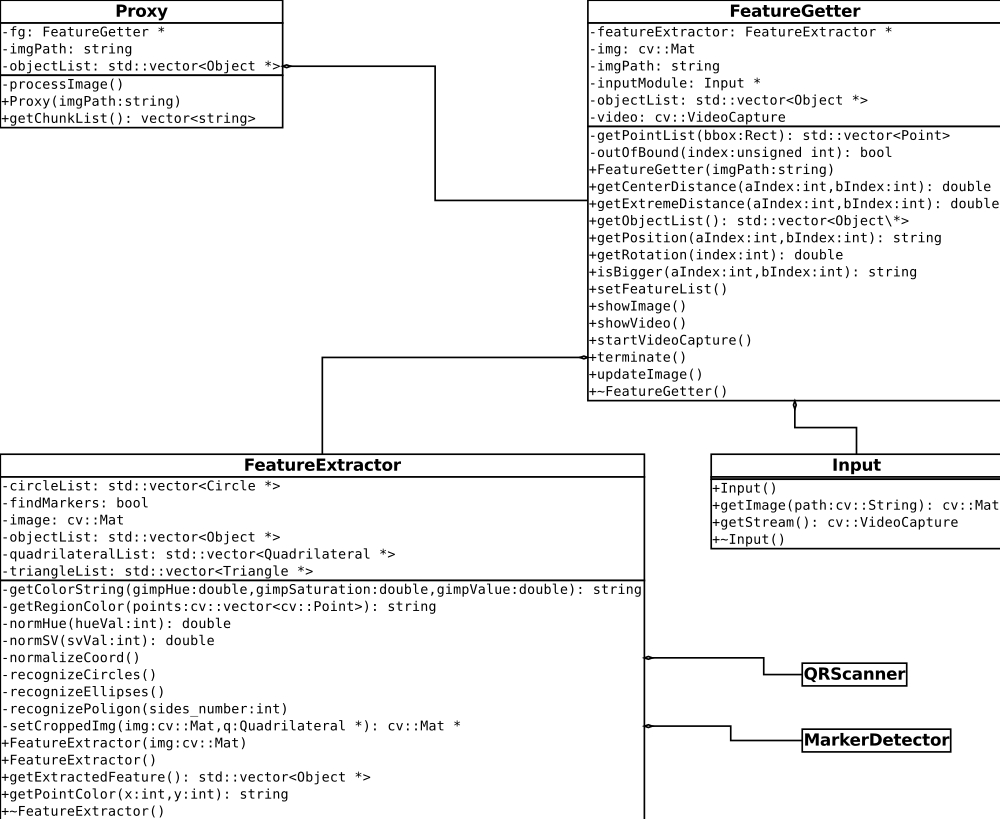
\includegraphics[width=\textwidth*\real{0.9}]{images/ch_06/fe.jpg}
		    }
		  \end{center} 
		  \caption{\textit{Class diagram describing the implementation of the feature extraction part of the software}}  
		  \label{fig:impl_feat_extraction}
	 	\end{figure}	


		\subsection{Object Hierarchy}
		As it can be noticed comparing the diagram in figure \ref{fig:impl_hierarchy} with the diagram of the design at page \pageref{fig:HierarchyDesign}, the differences between the implementation and the project are minimal. 
		In fact, further classes have not been introduced; rather, the existing ones have been provided with additional parameters and methods, as, for example, the attributes \emph{color} and \emph{center}.
		According to the iterative development process, different parameters have been added at different moments of the development.
		\begin{figure}[h]
		  \begin{center} 
		    \fbox{	
		       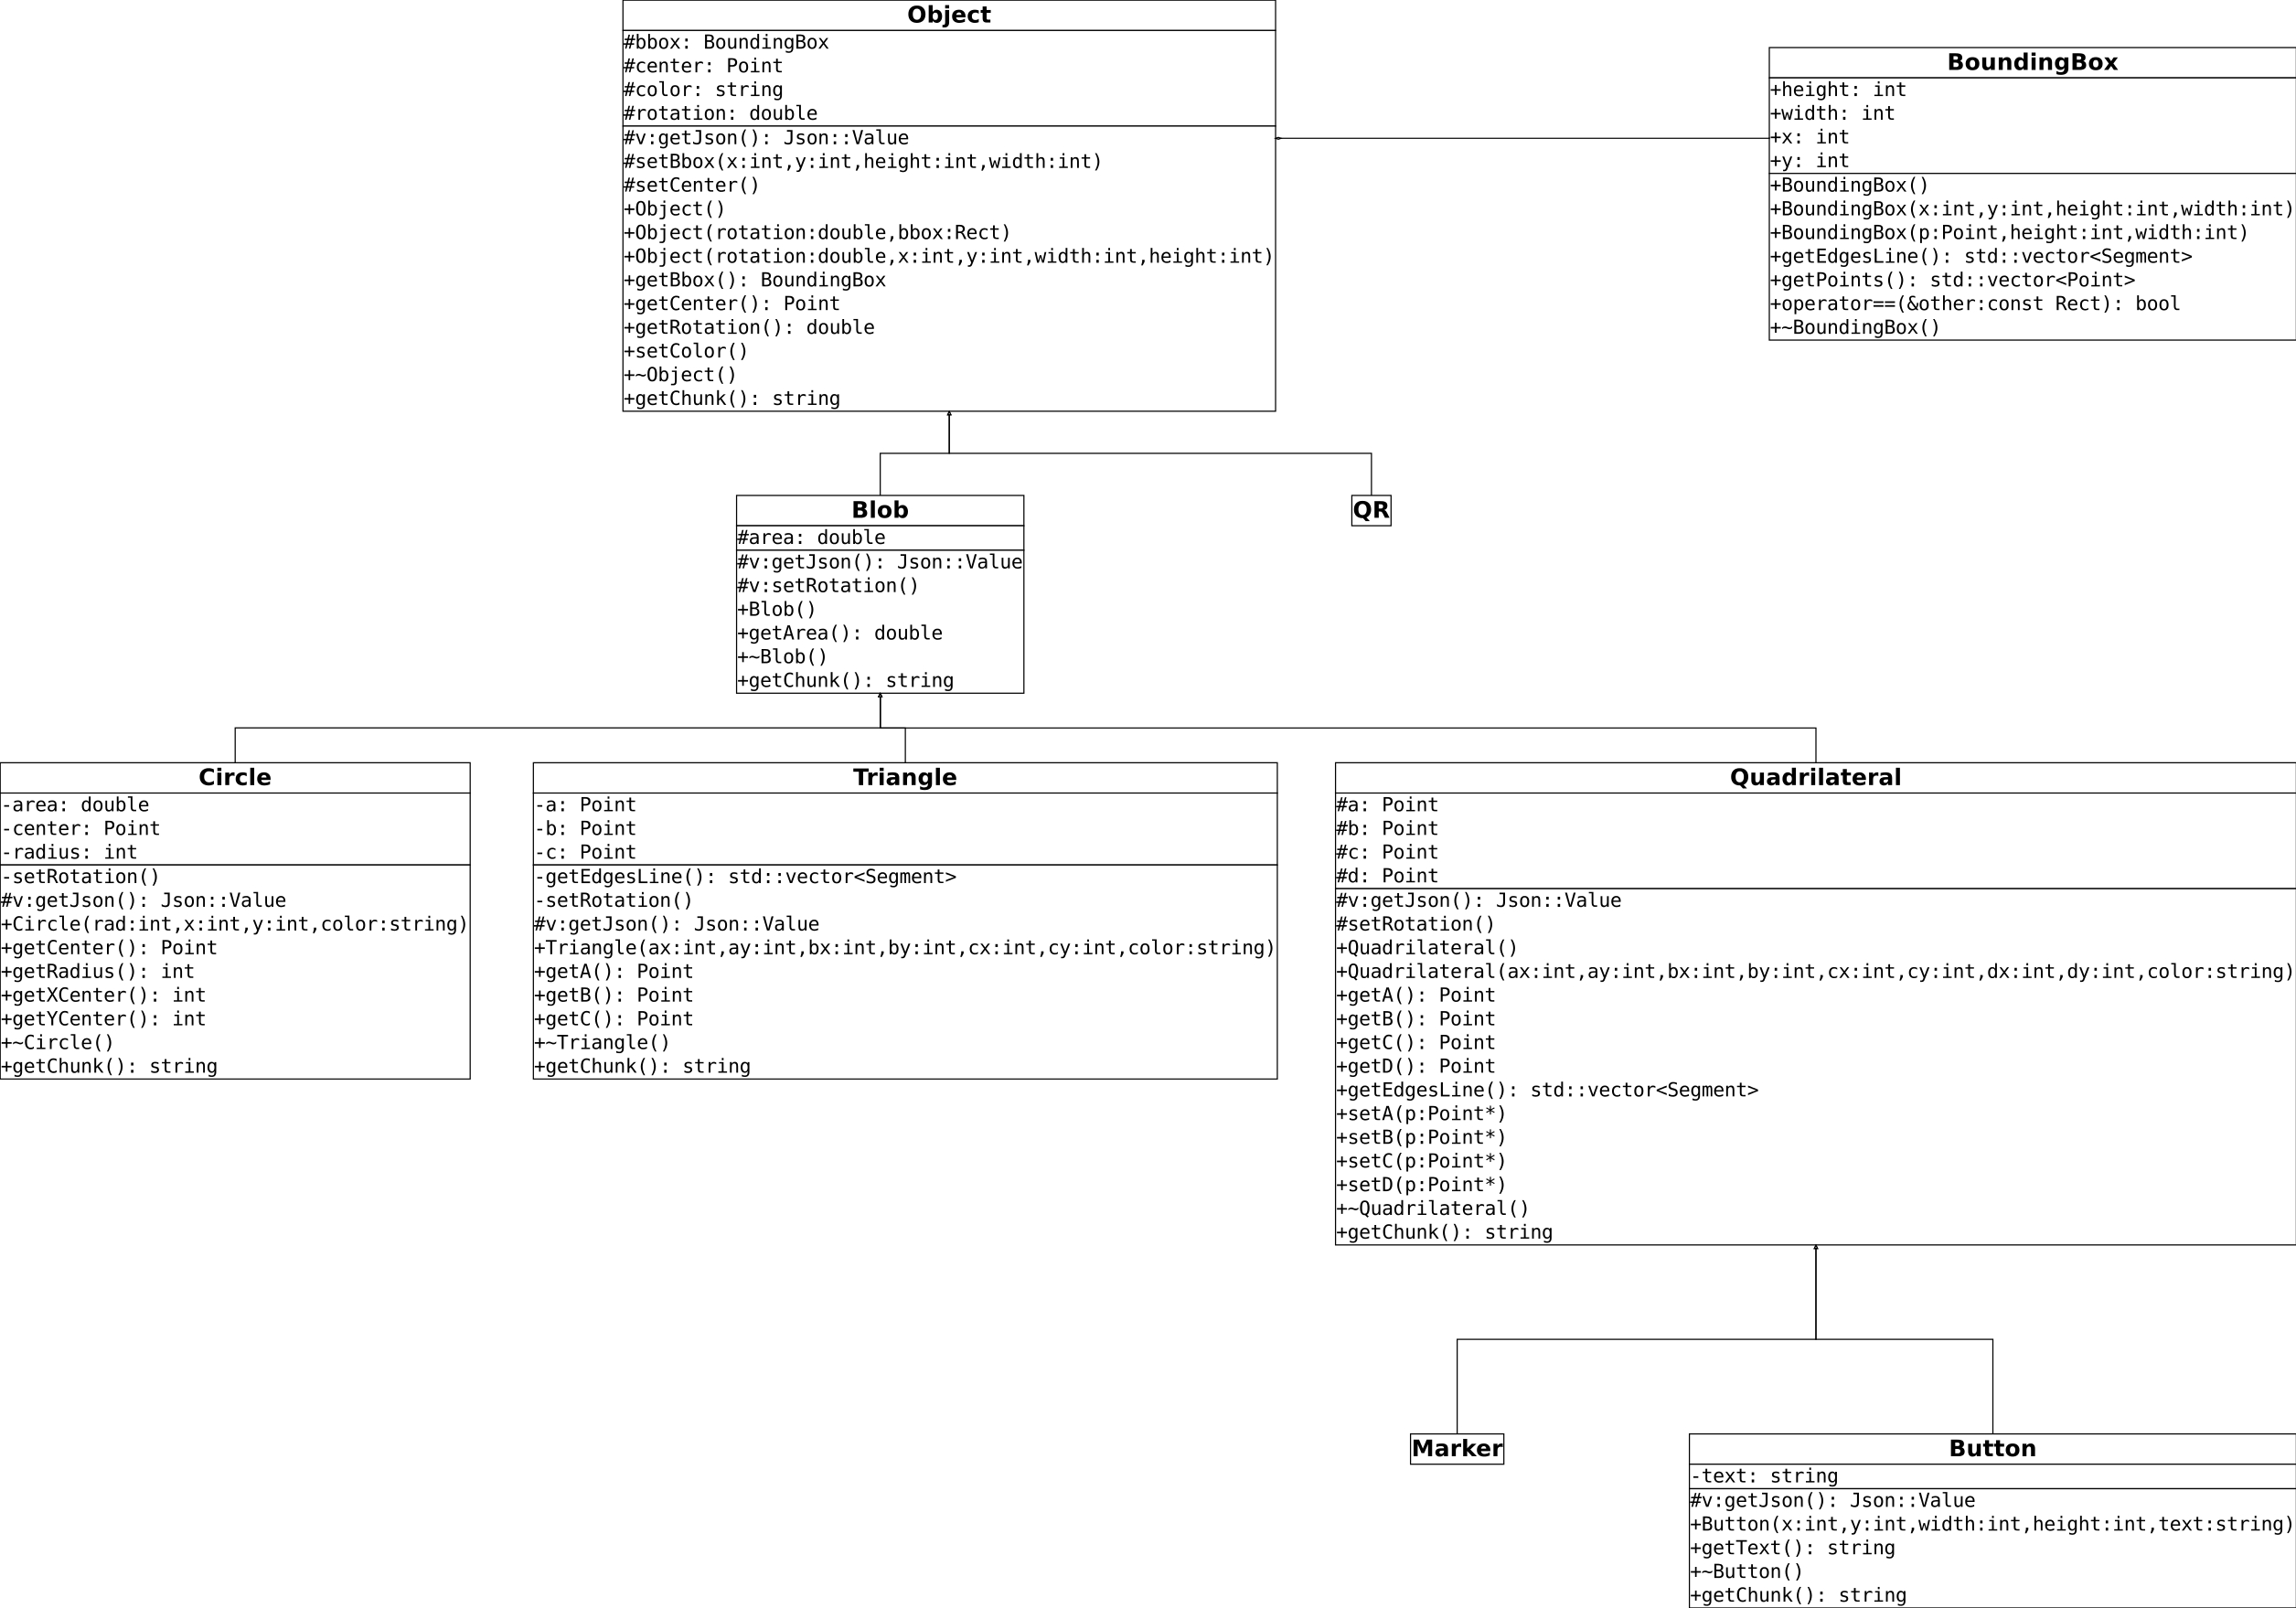
\includegraphics[width=\textwidth*\real{0.9}]{images/ch_06/hierarchy.jpg}
		    }
		  \end{center} 
		  \caption{\textit{Class diagram that shows the implementation of the object hierarchy}}  
		  \label{fig:impl_hierarchy}
	 	\end{figure}

	

		\subsection{Utility Part}
		The classes which form the utility parts of the software are divided in two categories: the exception classes and the ones representing all the other utilities. 
		To these, two modules containing functions are added. 
		Figure \ref{fig:impl_utility} shows a class diagram containing all the classes that constitute this part of the software. 
		The modules, as not classes, can not be shown in the diagram.

		\begin{figure}[h]
		  \begin{center} 
		    \fbox{	
		       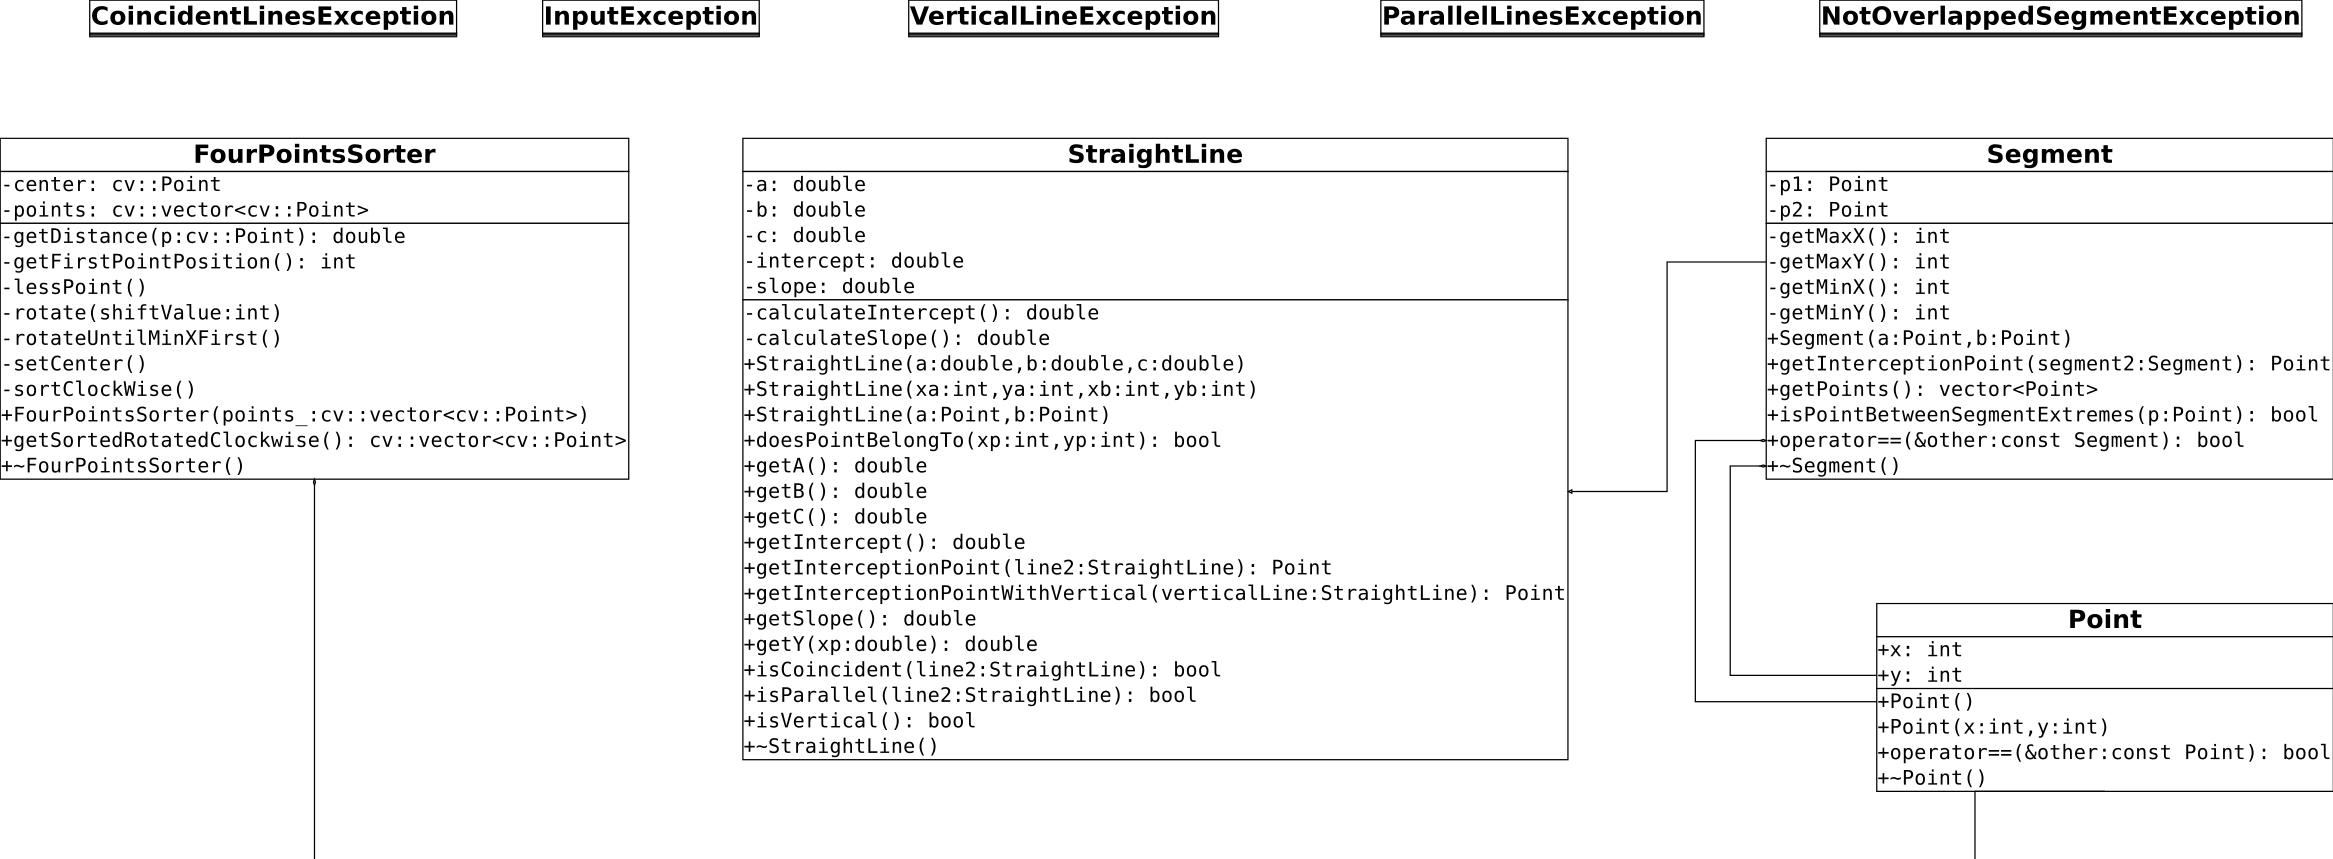
\includegraphics[width=\textwidth*\real{0.9}]{images/ch_06/utility.jpg}
		    }
		  \end{center} 
		  \caption{\textit{Class diagram showing the utility part of the software}}  
		  \label{fig:impl_utility}
	 	\end{figure}

		Classes \emph{InputException}, \emph{NotOverlappedSegmentException}, \emph{ParallelLinesException}, \emph{VerticalLineException} and \emph{CoincidentLinesException} are the exceptions classes. 
		As such, they are used to handle all the anomalous or exceptional events occurring at run-time.	
	
		\emph{StraightLine}, \emph{Segment} and \emph{Point} represent geometrical entities. These elements serve as basic structures for creating the objects in the hierarchy and making evaluations between couples of objects.
		Such evaluations can be both qualitative and quantitative, as, for example, the distances between the centers of two objects or the relative positions of one object in respect with another.
		
		\emph{FourPointsSorter} and the function modules contain the basic methods which are fundamental for all the operations executed by all the other classes of the software.
		For reasons of completeness the prototypes of the functions are listed in appendix \ref{appA}.

		


\begin{comment}
		The utility part is composed by the classes \emph{InputException}, \emph{NotOverlappedSegmentException}, \emph{ParallelLinesException}, \emph{VerticalLineException}, \emph{CoincidentLinesException}, \emph{FourPointsSorter}, \emph{StraightLine}, \emph{Segment}, \emph{Point} and another module containing functions. The latter, as it is not a class, is not included in the diagram in figure \ref{fig:impl_utility}. 

		\emph{InputException}, \emph{NotOverlappedSegmentException}, \emph{ParallelLinesException}, \emph{VerticalLineException} and \emph{CoincidentLinesException} are exceptions classes, used to handle all the anomalous or exceptional events occurring during the execution of the software. 

		\emph{StraightLine}, \emph{Segment} and \emph{Point} represent geometrical entities. Such elements are fundamental structures for creating the objects in the hierarchy and making evaluations between couples of objects.
		Such evaluations can be both qualitative and quantitative, as, for example, the distances between the centers of two objects or the relative positions of one object in respect with another.

		\emph{FourPointsSorter} and the function module contain the basic methods which are fundamental for all the operations executed by all the other classes of the software.

\end{comment}
		

		

	

	%\clearpage
 	%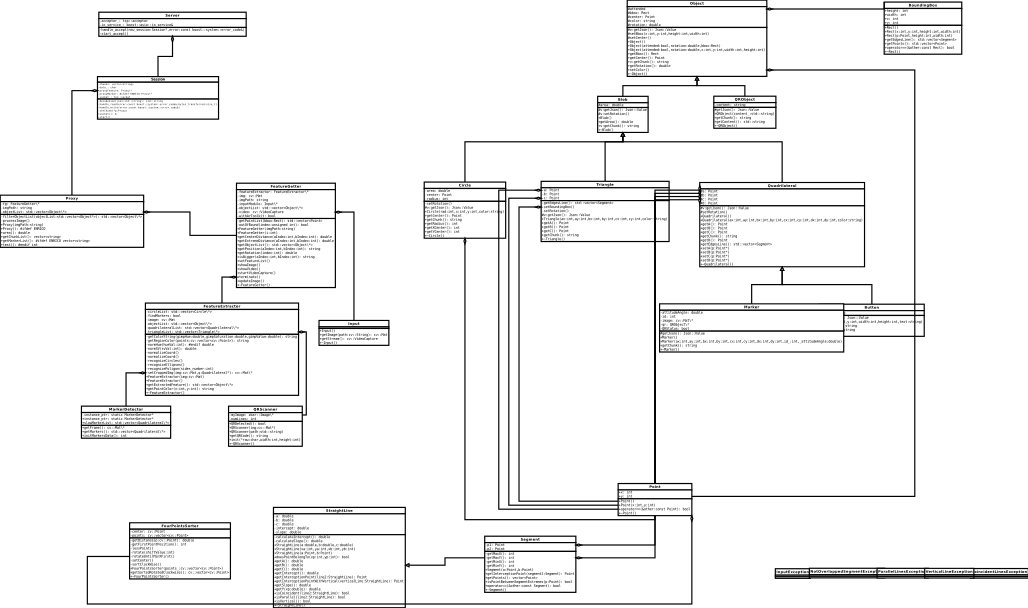
\includegraphics[angle=90,height=\textheight]{images/ch_06/implementation.jpg}\thispagestyle{empty}
\begin{comment}
	\pagestyle{empty}
	\begin{center} 	
	\fbox{	
		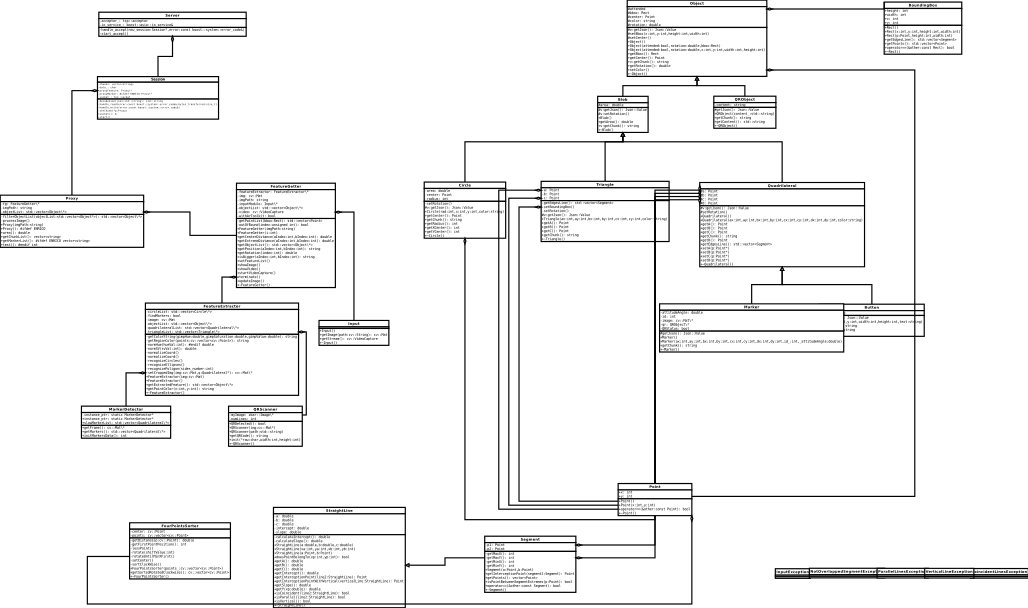
\includegraphics[angle=90,height=26cm]{images/ch_06/implementation.jpg}%\thispagestyle{empty}
	}
	%\caption{\textit{Class diagram illustrating a high level overview of the implementation}} 
	\label{fig:impl}
	\end{center}
\end{comment}	


	\section{Shape Recognition Extraction Algorithm} 	

	%\section{} 	

	\section{Testing}
\begin{comment}

	As it can be seen in the picture, the software is logically divided in the four main components introduced in the design chapter (see \ref{chDesign}).
%, respecting the in the design specifics described in chapter \ref{chDesign}. 
	Both the feature extraction part and the class hierarchy respect the design specifications, described in such chapter. The classes responsible for the communication with \mbox{ACT-R} and the utility part.
The communication with  and


	\newpage
	
	\begin{sidewaysfigure}[hbtp]
	   \thispagestyle{empty}	
 	   \centering
	   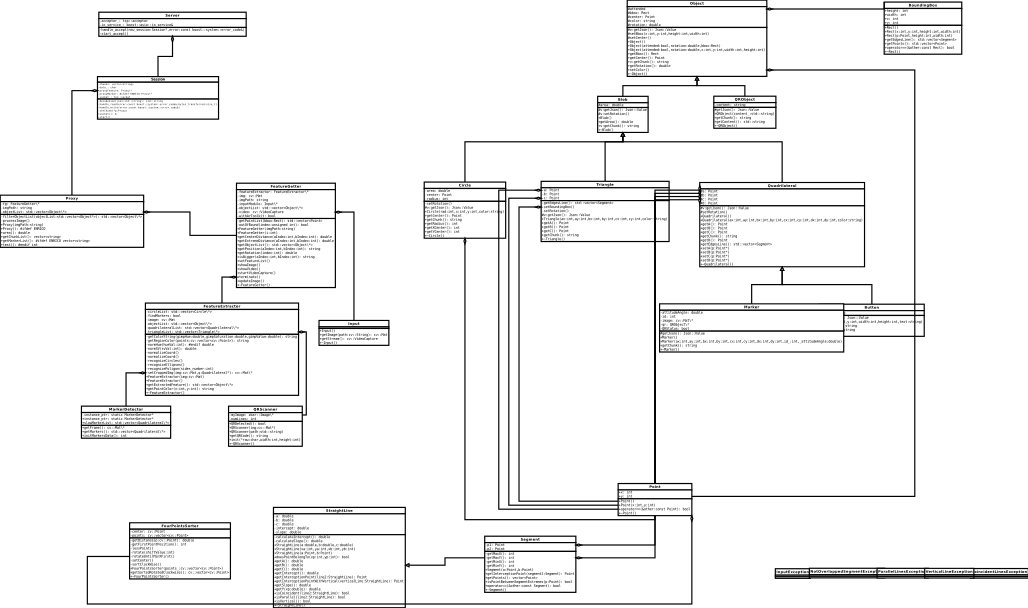
\includegraphics[height=\textheight]{images/ch_06/implementation.jpg}
	   
	  \caption{\textit{Class diagram illustrating the class hierarchy of the recognized objects}}  
	  \label{fig:HierarchyDesign}
 	\end{sidewaysfigure}

\newpage

\relax
	\AddToShipoutPicture*{ \\ \relax
	  \setlength{\unitlength}{1mm} 
	  \put(<10>, <10>){  
	    \makebox(0,0){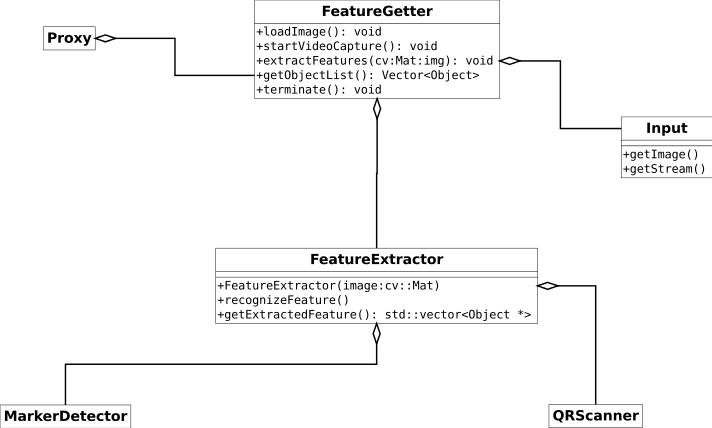
\includegraphics{images/ch_05/feature.png}}}} 
	ciao

	
\end{comment}

	%\section{COmmunication with ACT-R}
	%ciao

	\newpage
	\chapter{Conclusions}
	The objective of this work is to develop a software module which receives images as input and analyzes them by extracting particular information like the shapes they contain, their colors and their positions and communicates them to \mbox{ACT-R} when the cognitive architecture requests it. 
	The ultimate purpose of this is to create a vision module for the cognitive architecture in order to make its visual perception as similar as possible to human one.
	

	The developed software uses \mbox{OpenCV} library to implement the visual operations and communicates the information to \mbox{ACT-R} thanks to a client-server communication method. 
	This solution is simple, fast and allows to use a library which provides ready and tested functions for computer vision.  


	The software at the moment recognizes quadrilaterals, circles and rectangles and makes qualitative and quantitative evaluations about colors and relative positions and dimensions of the objects. 
	In particular, the tool is used in the Rush Hour experiment for analyzing the input image, extracting the list of objects it contains and communicating it to \mbox{ACT-R}. 
	In this way the cognitive architecture does not start working from a list of objects but it processes an image, even if indirectly.
	This fact approaches the \mbox{ACT-R} perception to human one. 	
		

	The restricted number of features offered by the visual module at the moment represent the biggest limit of this solution.
	However, it is enough to add new functions to this tool in order to extend more and more the scope of this module and use it increasingly together with \mbox{ACT-R}.


	In order to adapt the system to be able to work with other experiments, the first improvements that can be done are adding the recognition of new kinds of shape, for example ellipses, and a tool for \emph{{Optical Character Recognition\footnote{An Optical Character Recognition, also known as OCR, is a software which recognizes and decodes text in images.}}}.
	In fact, at the moment, images used in the experiments conducted with the cognitive architecture, in general are quite simple.
	They normally contain only simple shapes and may include some text.
	The introduction of methods for recognizing new shapes and texts make the system more scalable with the definition  of new experiments that need to process images.


	Adding new functions for object recognition can provide \mbox{ACT-R} with the ability of processing images directly in the real world. 
	This can lead to interesting applications in many research fields, including the spatial reasoning. 
	For example, the team developed a system for robots navigation with landmarks inside buildings. 
	The robot, together with the vision module, is able to identify a landmark, move close to it, decode the information it stores and send it to \mbox{ACT-R}, which can then communicate the robot how to behave.


 




\begin{comment}	
	aggiungere:
		riconoscimento ellissi
		riconoscimento testo

		introdurre il flusso video --> predisposto
	
		migliorare le performance dell'algoritmo in modo tale che la shape detection sia utilizzata in tempo reale pnell'ambito della navigazione con robot.
\end{comment}	



\pagenumbering{roman}


\newpage
\clearpage
\appendix
%\input{Chapters/appendice}
\newpage
\clearpage



%******************************************************************
% Materiale Finale
%******************************************************************
%******************************************************************
%References (two methods in Latex, this (bibTex) with the databe is the best
%******************************************************************
\cleardoublepage
\phantomsection						%gives hyperref something to hold on to when making the link.
\addcontentsline{toc}{chapter}{References}
\bibliographystyle{alpha}				%scelgo come formattare la biblio (abbrv abbrevia i nomi propri. plain non li abbrevia. Ce ne sono un sacco).
\bibliography{beginningEnding/database_references} 	%database dove prendere le info  
\nocite{*}						%stampa TUTTO quello presente nella banca dati, altrimenti solo la roba citata nella tesi

%NB in kile bisogna aggiungere BibTex al QuickBuild per far compilare la bibliografia. Metterlo subito dopo Latex.

\newpage										
\clearpage


\end{document}
